\documentclass[10pt,pdf,hyperref={unicode}]{beamer}
\usetheme{Antibes}
\usepackage[utf8]{inputenc}
\usepackage[T2A]{fontenc}
\usepackage[english,russian]{babel}
\usepackage{graphicx}

\title[Турнир Архимеда по программированию 2015] % (optional, only for long titles)
{Турнир Архимеда по программированию 2015}
\subtitle{Разбор задач}
\author[Мингалёв, Игнатьева] % (optional, for multiple authors)
{{Олег~Мингалёв\inst{1} \and Елизавета~Игнатьева\inst{2}} \\ {Александр~Тимин\inst{3} \and Валерия~Петрова\inst{4}}}
\institute[Universities Here and There] % (optional)
{
  \inst{1}%
  ГБОУ <<Физматшкола 2007>>, г. Москва
  \and
  \inst{2}%
  Московский Физико-Технический Институт, г. Долгопрудный
  \and
  \inst{3}%
  ООО <<Яндекс>>, г. Москва
  \and
  \inst{4}
  Центр онлайн-обучения <<Фоксфорд>>, г. Санкт-Петербург
}
\date[KPT 2015] % (optional)
{\url{http://archimedes-contest.org/}\\
26 апреля 2015 --- 3 мая 2015}

\begin{document}
  \frame{\titlepage}
  \section{Разбор задач}
  \section{Задача <<Нью-Кэпитал>>}


\begin{frame}
    \begin{center}
        \Huge Задача <<Нью-Кэпитал>>
    \end{center}
    ~\\~\\
    \begin{center}
        Автор задачи: Олег~Мингалёв\\
        Автор условия: Елизавета~Игнатьева\\
        Автор тестов: Олег~Мингалёв
    \end{center}
\end{frame}

\subsection{Постановка задачи}

\begin{frame}
    \frametitle{Постановка задачи}

    \begin{itemize}
        \item На плоскости отмечены две точки $S$ и $F$: $(S_X, S_Y)$ и $(F_X, F_Y)$.
        \item Из точек с чётными $X$-координатами разрешено двигаться на $1$~влево.
        \item Из точек с нечётными $X$-координатами разрешено двигаться на $1$~вправо.
        \item Из точек с чётными $Y$-координатами разрешено двигаться на $1$~вниз.
        \item Из точек с нечётными $Y$-координатами разрешено двигаться на $1$~верх.
        \item Другие ходы запрещены
        \item За какое минимальное число ходов из точки $S$ можно попасть в точку $F$?
    \end{itemize}
\end{frame}

\subsection{Решение}

\begin{frame}
    \frametitle{Разбор случаев}

    \begin{itemize}
        \item Рассмотрим решение для случая, в котором $S_X$ и $S_Y$ чётные, остальные случаи разбираются аналогично.
    \end{itemize}
\end{frame}

\begin{frame}
    \frametitle{Разбор случаев}

    \begin{itemize}
        \item Если бы из точек можно было ходить в любую сторону, то ответом на задачу было бы число $D = |S_X-F_X| + |S_Y-F_Y|$.
        \item Понятно, что в решаемой нами задаче ответ не может быть меньше, чем $D$.
        \item Назовём штрафом точки $A: (X, Y)$ разность минимального количества ходов, необходимого для достижения точки~$A$ из точки~$S$ и величины $|S_X-Y| + |S_Y-Y|$.
    \end{itemize}
\end{frame}

\begin{frame}
    \frametitle{Разбор случаев}

    \begin{itemize}
        \item Нарисуем все кратчайшие пути из $S$.
    \end{itemize}
    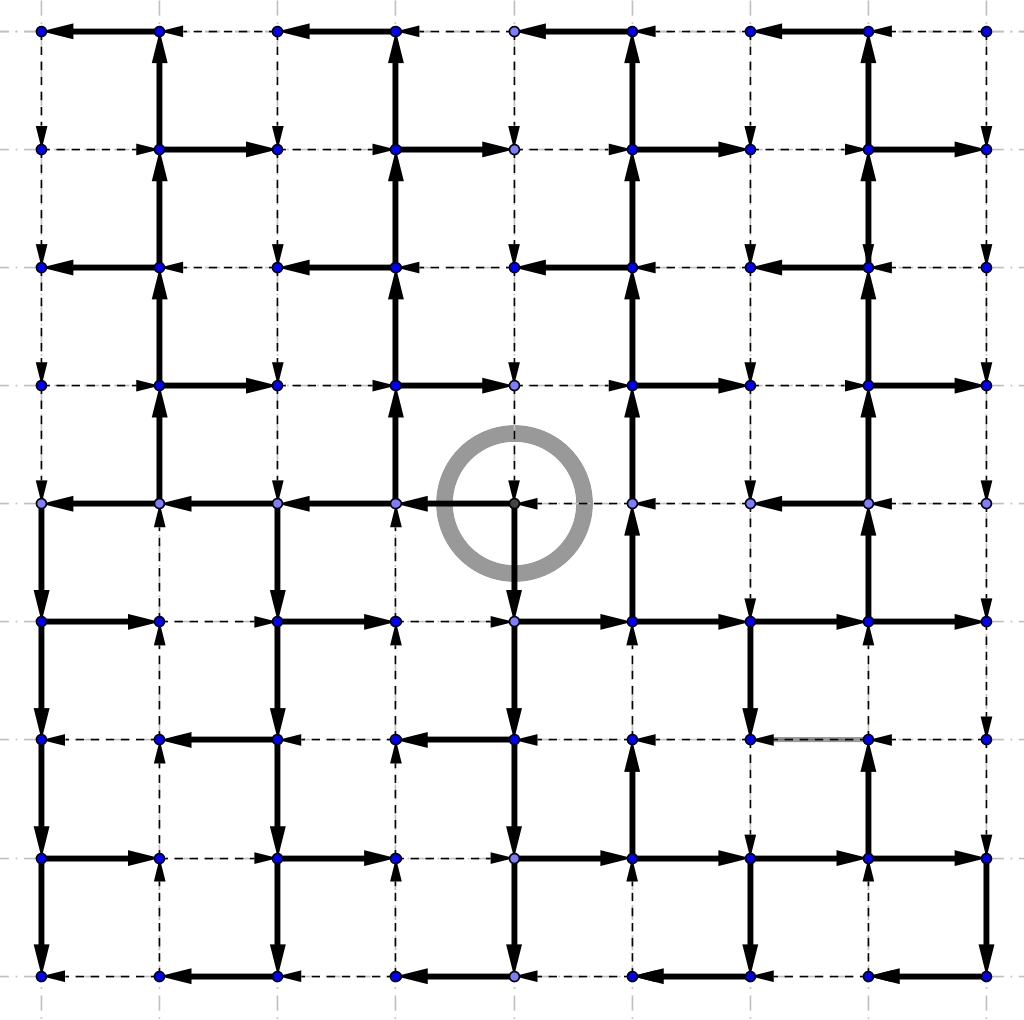
\includegraphics[scale=0.6]{manhattan/pics/even_even.png}
\end{frame}

\begin{frame}
    \frametitle{Разбор случаев}

    \begin{itemize}
        \item Для каждой точки посчитаем её штраф (на рисунке штраф, равный $0$, отмечен зелёным цветом, равный $2$ --- синим, равный $4$ --- красным.
    \end{itemize}
    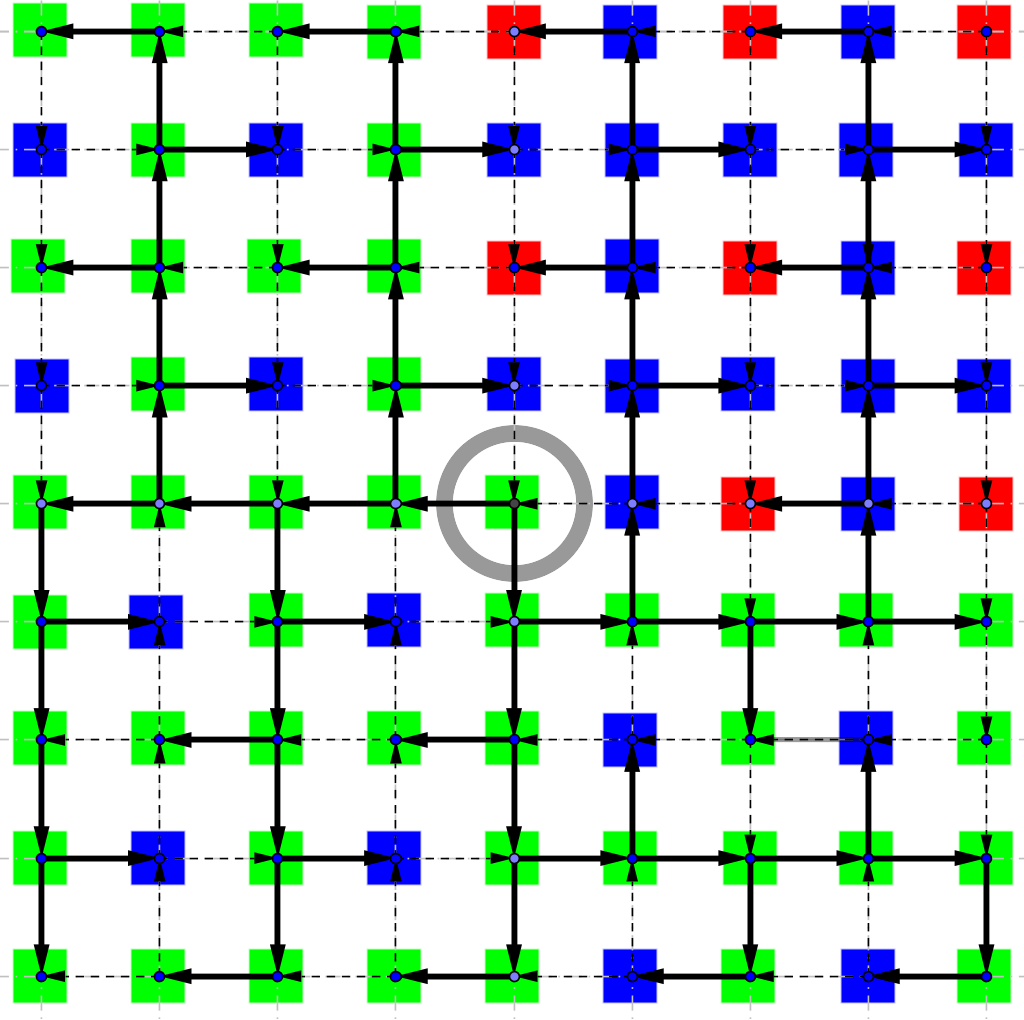
\includegraphics[scale=0.6]{manhattan/pics/even_even_penalty.png}
\end{frame}

\begin{frame}
    \frametitle{Разбор случаев}

    \begin{itemize}
        \item Заметим, что плоскость разбивается на четыре области, в каждой из которых штраф точки зависит только от чётности её координат.
    \end{itemize}
    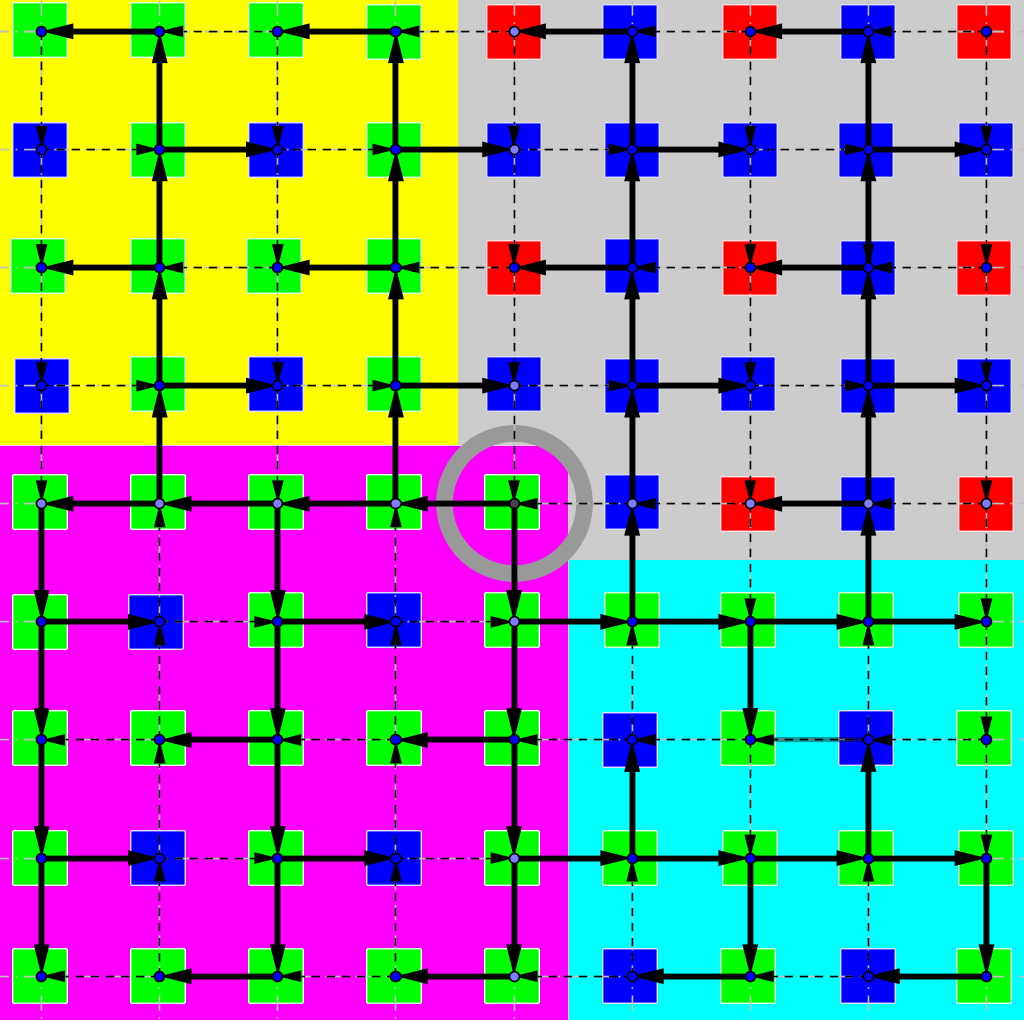
\includegraphics[scale=0.6]{manhattan/pics/even_even_regions.png}
\end{frame}

\begin{frame}
    \frametitle{Разбор случаев}

    \begin{itemize}
        \item Проверить, в какой области лежит точка~$F$ относительно точки~$S$.
        \item Посчитать её штраф в зависимости от полученной области и чётности координат.
        \item Прибавить к штрафу величину $|S_X-F_X| + |S_Y-F_Y|$.
        \item Это и есть ответ.
        \item Для остальных случаев, когда $S_X$ или $S_Y$ нечётные, рассуждения полностью аналогичны.
    \end{itemize}
\end{frame}

\begin{frame}
    \frametitle{Поиск в ширину}

    \begin{itemize}
        \item Можно было честно искать кратчайшее расстояние между точками с помощью, например, алгоритма поиска в ширину.
        \item Подробнее --- например, на сайте \url{http://informatics.msk.ru/} в разделе <<Алгоритмы на графах>>.
    \end{itemize}
\end{frame}

\begin{frame}
    \begin{center}
        \Huge Вопросы?
    \end{center}
\end{frame}

  \section{Задача <<Нью-Кэпитал>>}


\begin{frame}
    \begin{center}
        \Huge Задача <<Нью-Кэпитал>>
    \end{center}
    ~\\~\\
    \begin{center}
        Автор задачи: Олег~Мингалёв\\
        Автор условия: Елизавета~Игнатьева\\
        Автор тестов: Олег~Мингалёв
    \end{center}
\end{frame}

\subsection{Постановка задачи}

\begin{frame}
    \frametitle{Постановка задачи}

    \begin{itemize}
        \item На плоскости отмечены две точки $S$ и $F$: $(S_X, S_Y)$ и $(F_X, F_Y)$.
        \item Из точек с чётными $X$-координатами разрешено двигаться на $1$~влево.
        \item Из точек с нечётными $X$-координатами разрешено двигаться на $1$~вправо.
        \item Из точек с чётными $Y$-координатами разрешено двигаться на $1$~вниз.
        \item Из точек с нечётными $Y$-координатами разрешено двигаться на $1$~верх.
        \item Другие ходы запрещены
        \item За какое минимальное число ходов из точки $S$ можно попасть в точку $F$?
    \end{itemize}
\end{frame}

\subsection{Решение}

\begin{frame}
    \frametitle{Разбор случаев}

    \begin{itemize}
        \item Рассмотрим решение для случая, в котором $S_X$ и $S_Y$ чётные, остальные случаи разбираются аналогично.
    \end{itemize}
\end{frame}

\begin{frame}
    \frametitle{Разбор случаев}

    \begin{itemize}
        \item Если бы из точек можно было ходить в любую сторону, то ответом на задачу было бы число $D = |S_X-F_X| + |S_Y-F_Y|$.
        \item Понятно, что в решаемой нами задаче ответ не может быть меньше, чем $D$.
        \item Назовём штрафом точки $A: (X, Y)$ разность минимального количества ходов, необходимого для достижения точки~$A$ из точки~$S$ и величины $|S_X-Y| + |S_Y-Y|$.
    \end{itemize}
\end{frame}

\begin{frame}
    \frametitle{Разбор случаев}

    \begin{itemize}
        \item Нарисуем все кратчайшие пути из $S$.
    \end{itemize}
    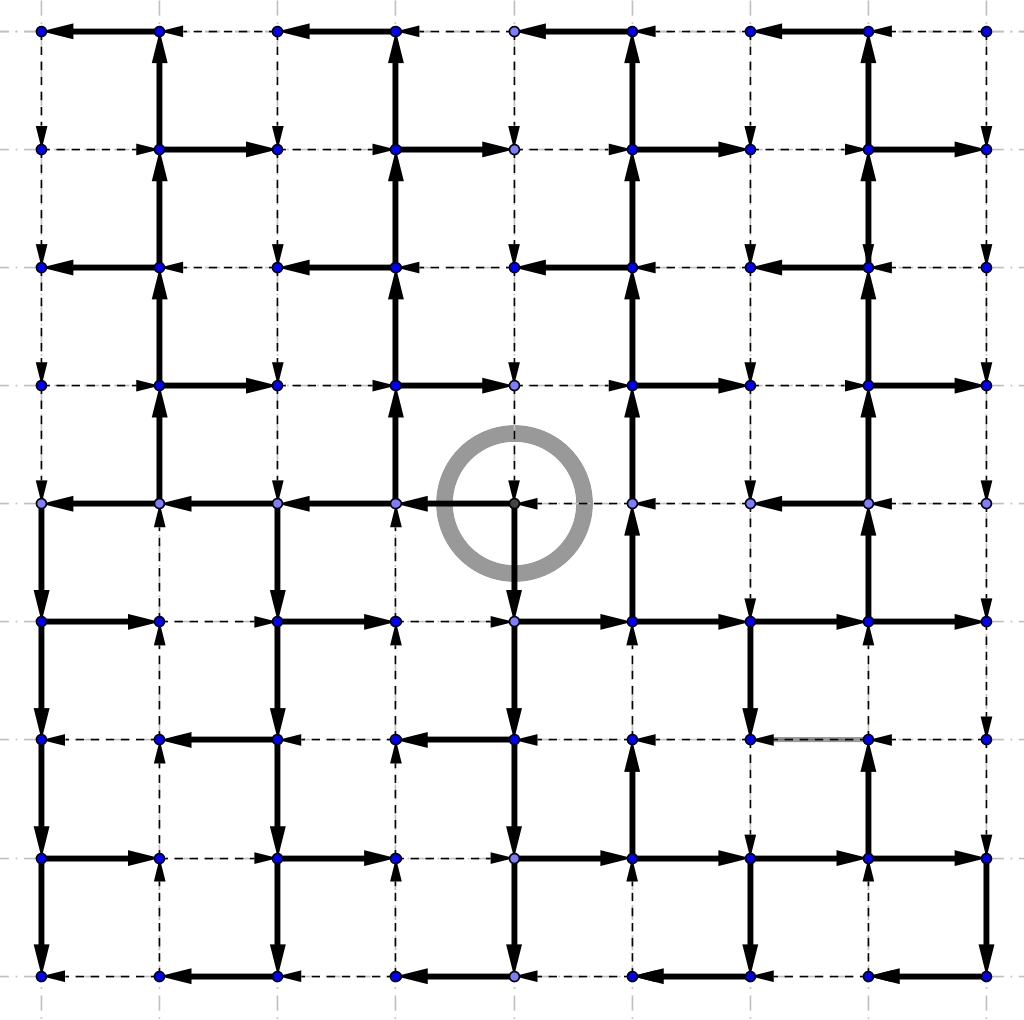
\includegraphics[scale=0.6]{manhattan/pics/even_even.png}
\end{frame}

\begin{frame}
    \frametitle{Разбор случаев}

    \begin{itemize}
        \item Для каждой точки посчитаем её штраф (на рисунке штраф, равный $0$, отмечен зелёным цветом, равный $2$ --- синим, равный $4$ --- красным.
    \end{itemize}
    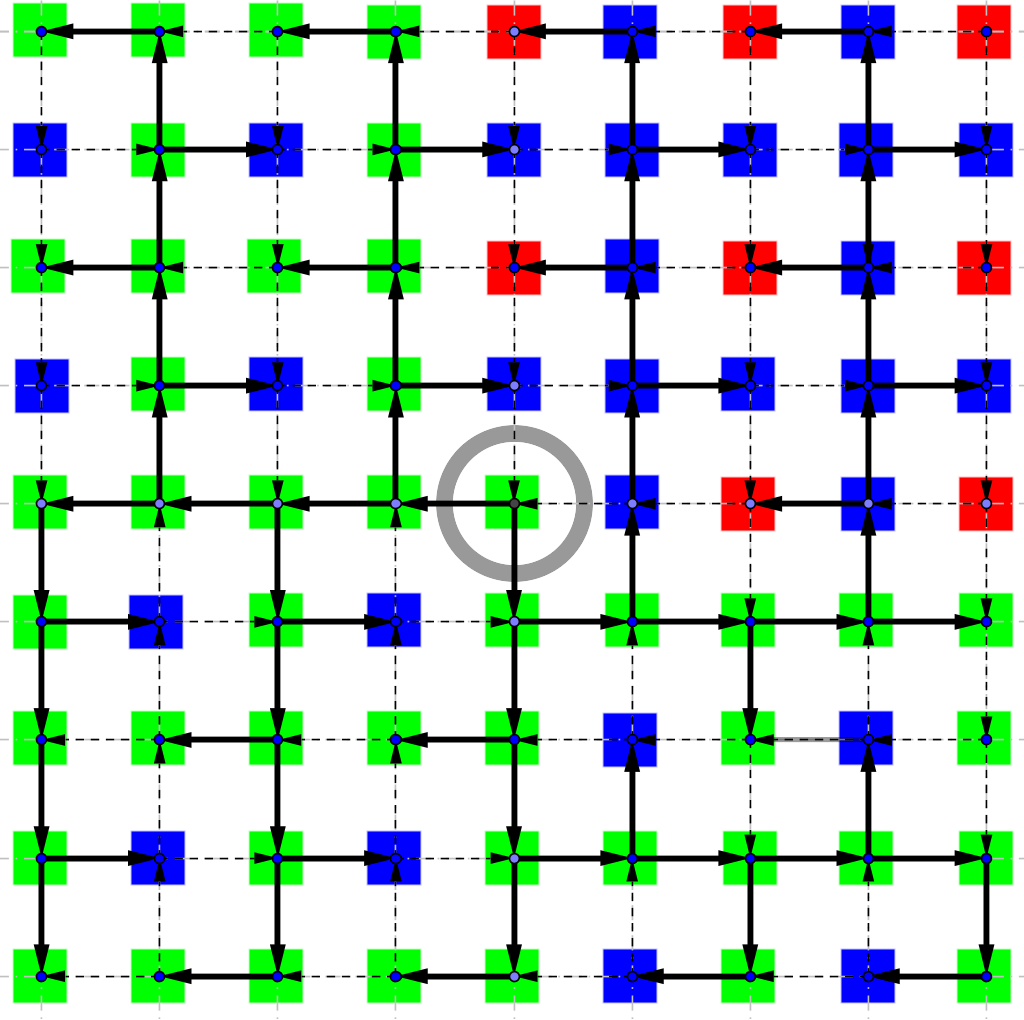
\includegraphics[scale=0.6]{manhattan/pics/even_even_penalty.png}
\end{frame}

\begin{frame}
    \frametitle{Разбор случаев}

    \begin{itemize}
        \item Заметим, что плоскость разбивается на четыре области, в каждой из которых штраф точки зависит только от чётности её координат.
    \end{itemize}
    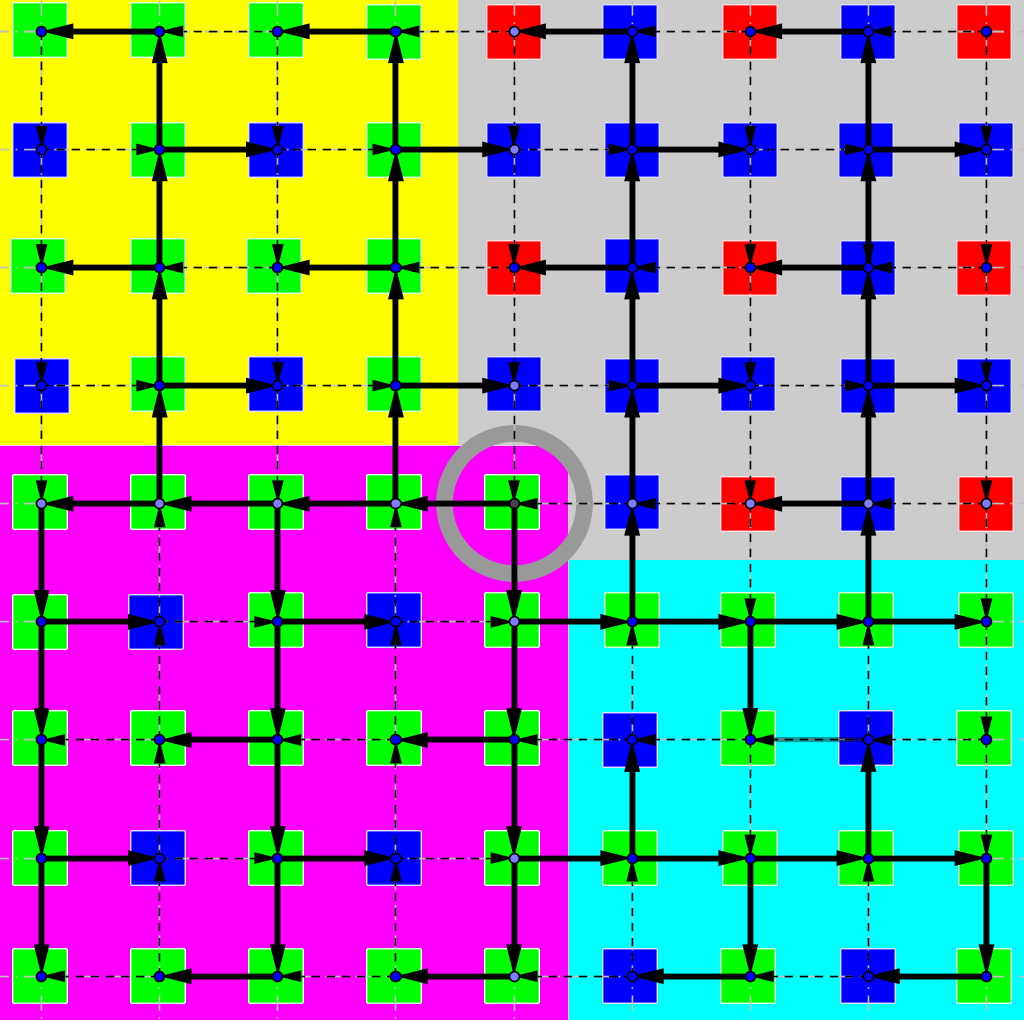
\includegraphics[scale=0.6]{manhattan/pics/even_even_regions.png}
\end{frame}

\begin{frame}
    \frametitle{Разбор случаев}

    \begin{itemize}
        \item Проверить, в какой области лежит точка~$F$ относительно точки~$S$.
        \item Посчитать её штраф в зависимости от полученной области и чётности координат.
        \item Прибавить к штрафу величину $|S_X-F_X| + |S_Y-F_Y|$.
        \item Это и есть ответ.
        \item Для остальных случаев, когда $S_X$ или $S_Y$ нечётные, рассуждения полностью аналогичны.
    \end{itemize}
\end{frame}

\begin{frame}
    \frametitle{Поиск в ширину}

    \begin{itemize}
        \item Можно было честно искать кратчайшее расстояние между точками с помощью, например, алгоритма поиска в ширину.
        \item Подробнее --- например, на сайте \url{http://informatics.msk.ru/} в разделе <<Алгоритмы на графах>>.
    \end{itemize}
\end{frame}

\begin{frame}
    \begin{center}
        \Huge Вопросы?
    \end{center}
\end{frame}

  \section{Задача <<Нью-Кэпитал>>}


\begin{frame}
    \begin{center}
        \Huge Задача <<Нью-Кэпитал>>
    \end{center}
    ~\\~\\
    \begin{center}
        Автор задачи: Олег~Мингалёв\\
        Автор условия: Елизавета~Игнатьева\\
        Автор тестов: Олег~Мингалёв
    \end{center}
\end{frame}

\subsection{Постановка задачи}

\begin{frame}
    \frametitle{Постановка задачи}

    \begin{itemize}
        \item На плоскости отмечены две точки $S$ и $F$: $(S_X, S_Y)$ и $(F_X, F_Y)$.
        \item Из точек с чётными $X$-координатами разрешено двигаться на $1$~влево.
        \item Из точек с нечётными $X$-координатами разрешено двигаться на $1$~вправо.
        \item Из точек с чётными $Y$-координатами разрешено двигаться на $1$~вниз.
        \item Из точек с нечётными $Y$-координатами разрешено двигаться на $1$~верх.
        \item Другие ходы запрещены
        \item За какое минимальное число ходов из точки $S$ можно попасть в точку $F$?
    \end{itemize}
\end{frame}

\subsection{Решение}

\begin{frame}
    \frametitle{Разбор случаев}

    \begin{itemize}
        \item Рассмотрим решение для случая, в котором $S_X$ и $S_Y$ чётные, остальные случаи разбираются аналогично.
    \end{itemize}
\end{frame}

\begin{frame}
    \frametitle{Разбор случаев}

    \begin{itemize}
        \item Если бы из точек можно было ходить в любую сторону, то ответом на задачу было бы число $D = |S_X-F_X| + |S_Y-F_Y|$.
        \item Понятно, что в решаемой нами задаче ответ не может быть меньше, чем $D$.
        \item Назовём штрафом точки $A: (X, Y)$ разность минимального количества ходов, необходимого для достижения точки~$A$ из точки~$S$ и величины $|S_X-Y| + |S_Y-Y|$.
    \end{itemize}
\end{frame}

\begin{frame}
    \frametitle{Разбор случаев}

    \begin{itemize}
        \item Нарисуем все кратчайшие пути из $S$.
    \end{itemize}
    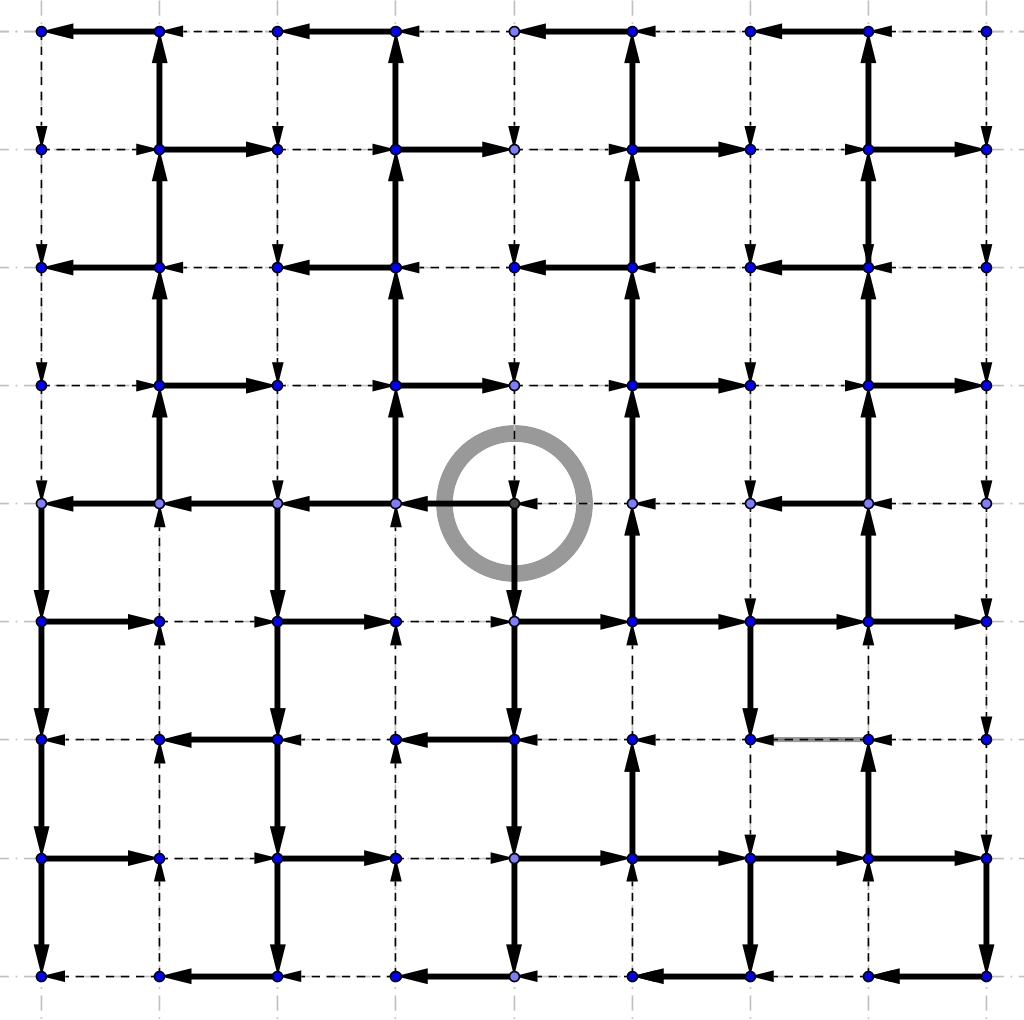
\includegraphics[scale=0.6]{manhattan/pics/even_even.png}
\end{frame}

\begin{frame}
    \frametitle{Разбор случаев}

    \begin{itemize}
        \item Для каждой точки посчитаем её штраф (на рисунке штраф, равный $0$, отмечен зелёным цветом, равный $2$ --- синим, равный $4$ --- красным.
    \end{itemize}
    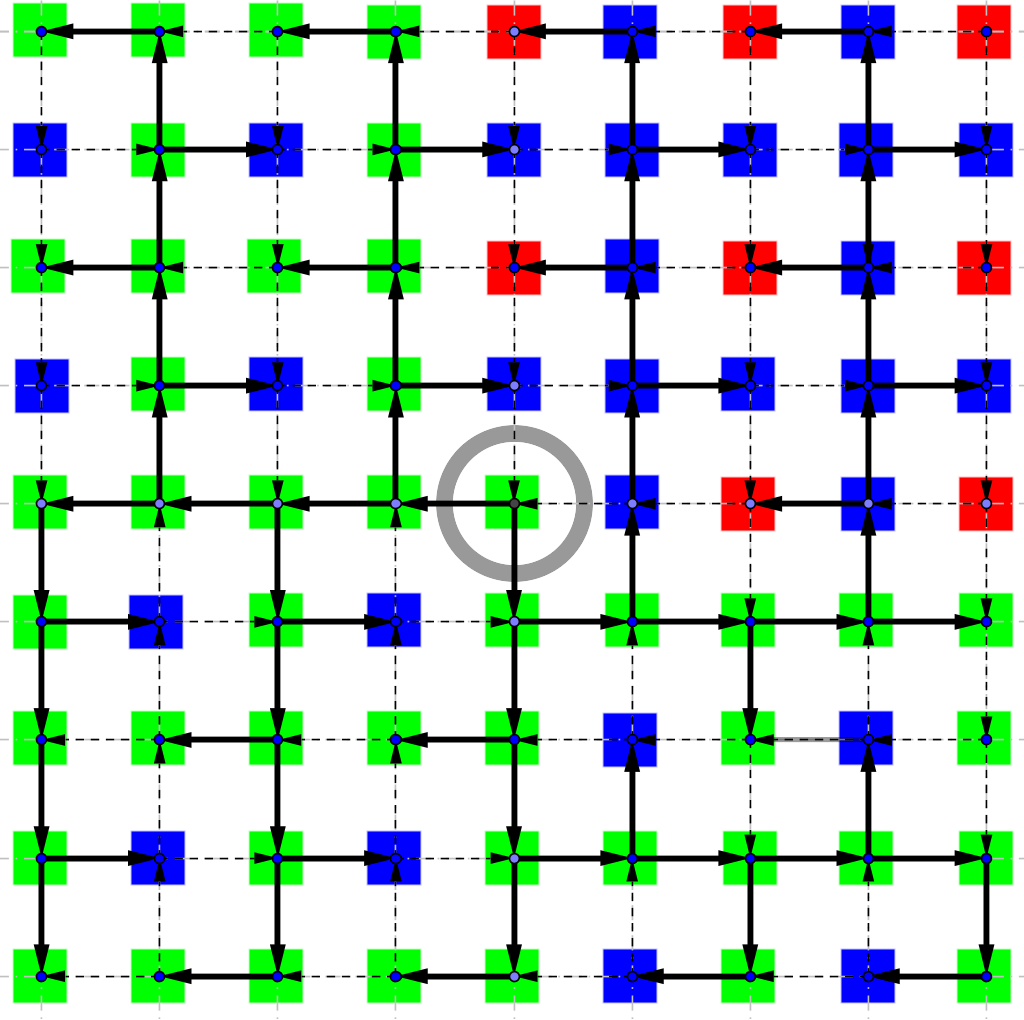
\includegraphics[scale=0.6]{manhattan/pics/even_even_penalty.png}
\end{frame}

\begin{frame}
    \frametitle{Разбор случаев}

    \begin{itemize}
        \item Заметим, что плоскость разбивается на четыре области, в каждой из которых штраф точки зависит только от чётности её координат.
    \end{itemize}
    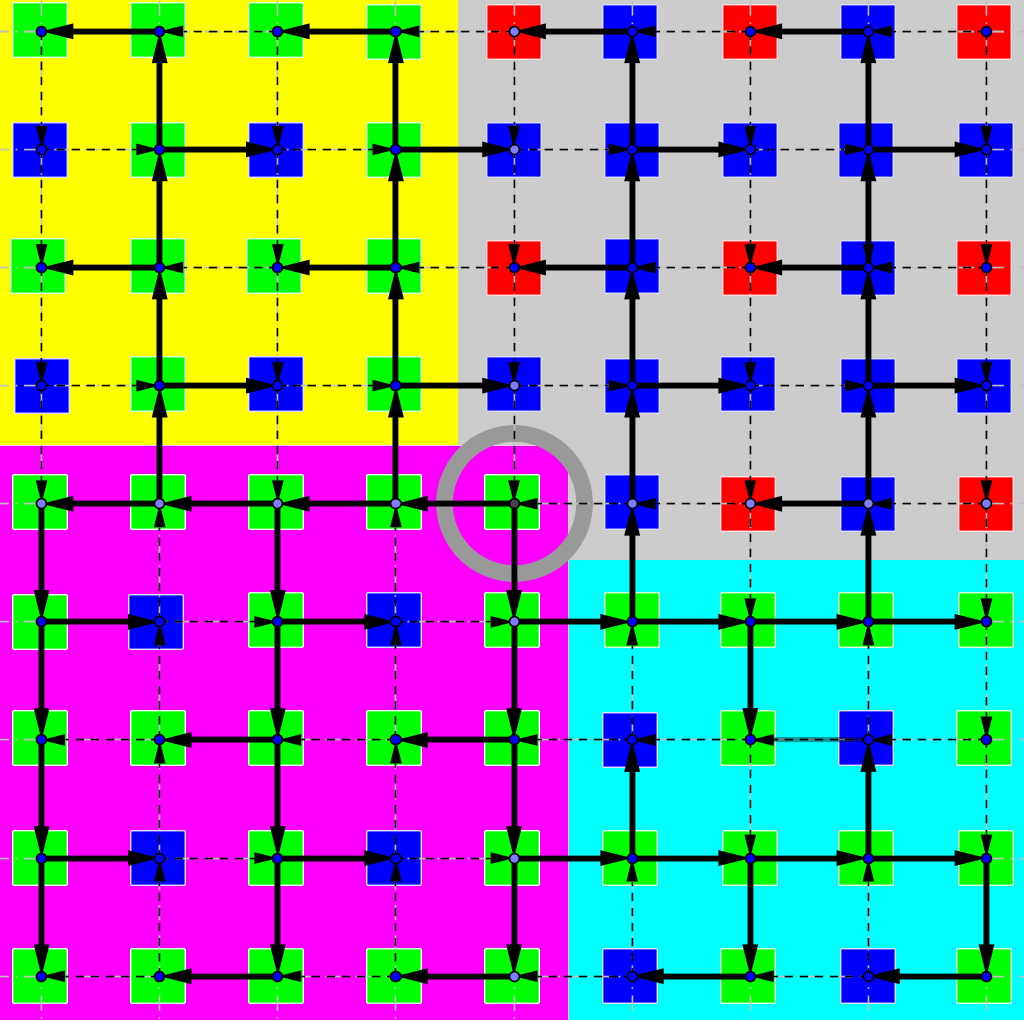
\includegraphics[scale=0.6]{manhattan/pics/even_even_regions.png}
\end{frame}

\begin{frame}
    \frametitle{Разбор случаев}

    \begin{itemize}
        \item Проверить, в какой области лежит точка~$F$ относительно точки~$S$.
        \item Посчитать её штраф в зависимости от полученной области и чётности координат.
        \item Прибавить к штрафу величину $|S_X-F_X| + |S_Y-F_Y|$.
        \item Это и есть ответ.
        \item Для остальных случаев, когда $S_X$ или $S_Y$ нечётные, рассуждения полностью аналогичны.
    \end{itemize}
\end{frame}

\begin{frame}
    \frametitle{Поиск в ширину}

    \begin{itemize}
        \item Можно было честно искать кратчайшее расстояние между точками с помощью, например, алгоритма поиска в ширину.
        \item Подробнее --- например, на сайте \url{http://informatics.msk.ru/} в разделе <<Алгоритмы на графах>>.
    \end{itemize}
\end{frame}

\begin{frame}
    \begin{center}
        \Huge Вопросы?
    \end{center}
\end{frame}

  \section{Задача <<Нью-Кэпитал>>}


\begin{frame}
    \begin{center}
        \Huge Задача <<Нью-Кэпитал>>
    \end{center}
    ~\\~\\
    \begin{center}
        Автор задачи: Олег~Мингалёв\\
        Автор условия: Елизавета~Игнатьева\\
        Автор тестов: Олег~Мингалёв
    \end{center}
\end{frame}

\subsection{Постановка задачи}

\begin{frame}
    \frametitle{Постановка задачи}

    \begin{itemize}
        \item На плоскости отмечены две точки $S$ и $F$: $(S_X, S_Y)$ и $(F_X, F_Y)$.
        \item Из точек с чётными $X$-координатами разрешено двигаться на $1$~влево.
        \item Из точек с нечётными $X$-координатами разрешено двигаться на $1$~вправо.
        \item Из точек с чётными $Y$-координатами разрешено двигаться на $1$~вниз.
        \item Из точек с нечётными $Y$-координатами разрешено двигаться на $1$~верх.
        \item Другие ходы запрещены
        \item За какое минимальное число ходов из точки $S$ можно попасть в точку $F$?
    \end{itemize}
\end{frame}

\subsection{Решение}

\begin{frame}
    \frametitle{Разбор случаев}

    \begin{itemize}
        \item Рассмотрим решение для случая, в котором $S_X$ и $S_Y$ чётные, остальные случаи разбираются аналогично.
    \end{itemize}
\end{frame}

\begin{frame}
    \frametitle{Разбор случаев}

    \begin{itemize}
        \item Если бы из точек можно было ходить в любую сторону, то ответом на задачу было бы число $D = |S_X-F_X| + |S_Y-F_Y|$.
        \item Понятно, что в решаемой нами задаче ответ не может быть меньше, чем $D$.
        \item Назовём штрафом точки $A: (X, Y)$ разность минимального количества ходов, необходимого для достижения точки~$A$ из точки~$S$ и величины $|S_X-Y| + |S_Y-Y|$.
    \end{itemize}
\end{frame}

\begin{frame}
    \frametitle{Разбор случаев}

    \begin{itemize}
        \item Нарисуем все кратчайшие пути из $S$.
    \end{itemize}
    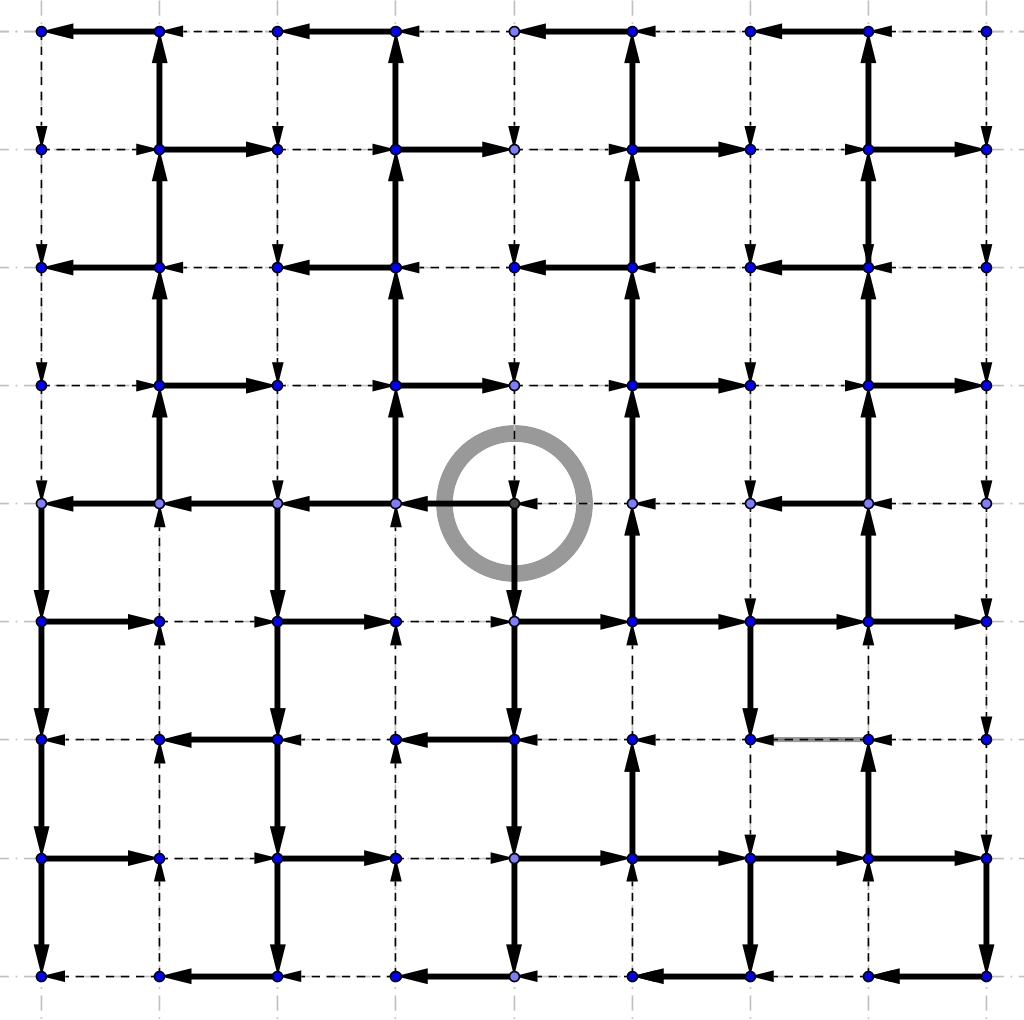
\includegraphics[scale=0.6]{manhattan/pics/even_even.png}
\end{frame}

\begin{frame}
    \frametitle{Разбор случаев}

    \begin{itemize}
        \item Для каждой точки посчитаем её штраф (на рисунке штраф, равный $0$, отмечен зелёным цветом, равный $2$ --- синим, равный $4$ --- красным.
    \end{itemize}
    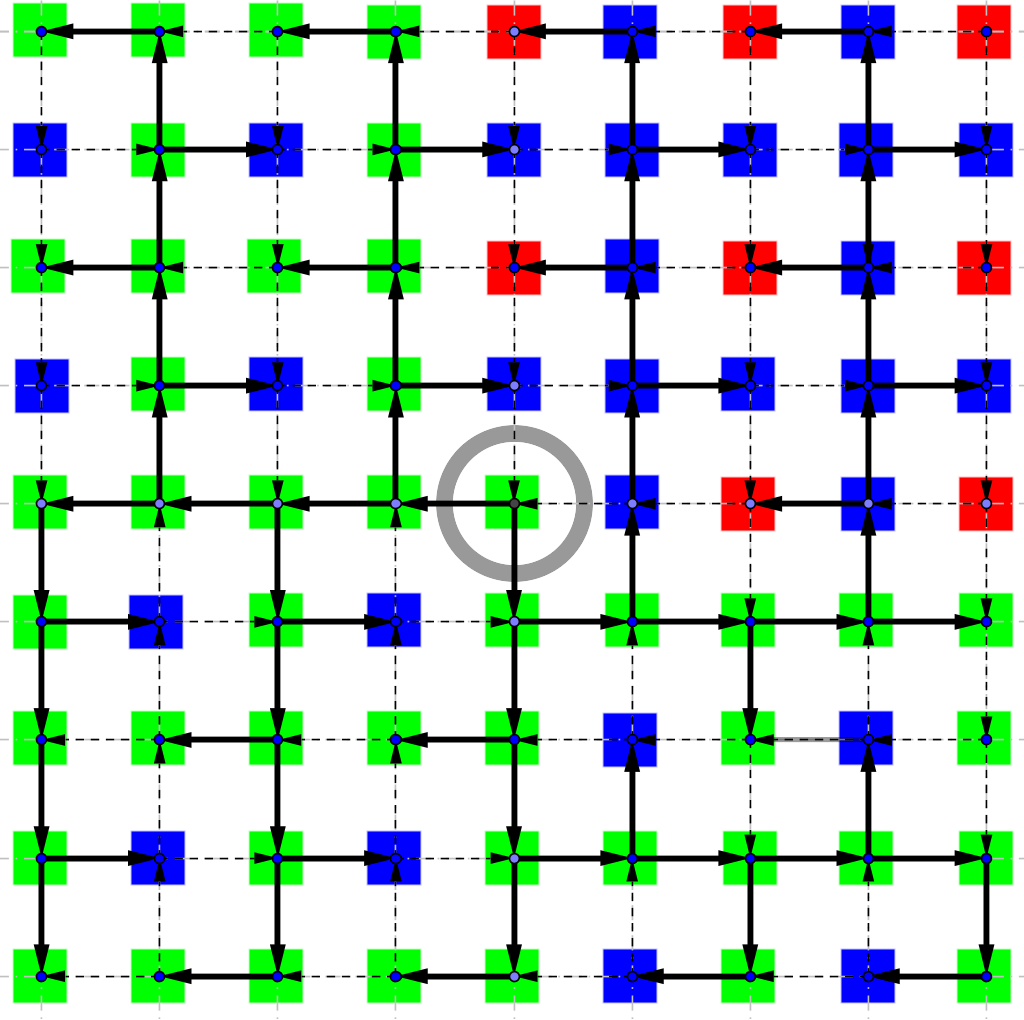
\includegraphics[scale=0.6]{manhattan/pics/even_even_penalty.png}
\end{frame}

\begin{frame}
    \frametitle{Разбор случаев}

    \begin{itemize}
        \item Заметим, что плоскость разбивается на четыре области, в каждой из которых штраф точки зависит только от чётности её координат.
    \end{itemize}
    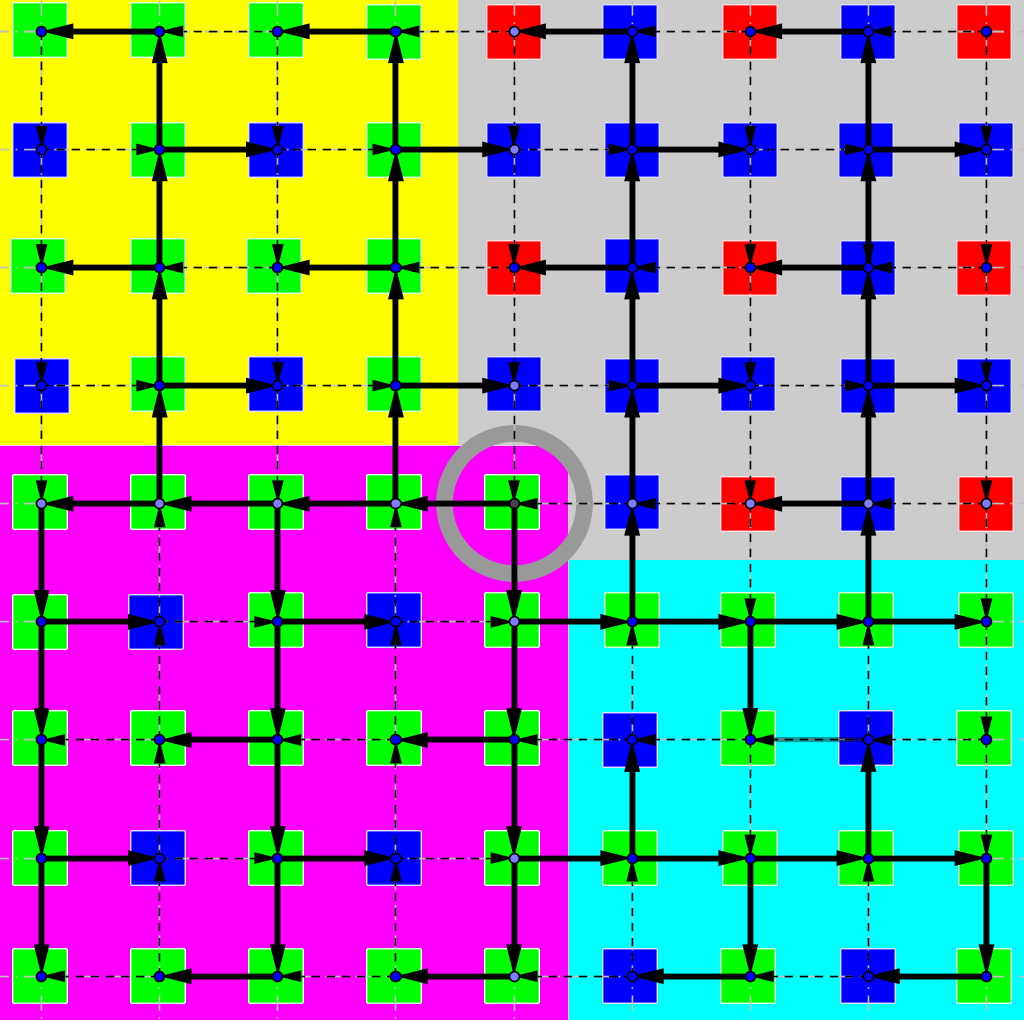
\includegraphics[scale=0.6]{manhattan/pics/even_even_regions.png}
\end{frame}

\begin{frame}
    \frametitle{Разбор случаев}

    \begin{itemize}
        \item Проверить, в какой области лежит точка~$F$ относительно точки~$S$.
        \item Посчитать её штраф в зависимости от полученной области и чётности координат.
        \item Прибавить к штрафу величину $|S_X-F_X| + |S_Y-F_Y|$.
        \item Это и есть ответ.
        \item Для остальных случаев, когда $S_X$ или $S_Y$ нечётные, рассуждения полностью аналогичны.
    \end{itemize}
\end{frame}

\begin{frame}
    \frametitle{Поиск в ширину}

    \begin{itemize}
        \item Можно было честно искать кратчайшее расстояние между точками с помощью, например, алгоритма поиска в ширину.
        \item Подробнее --- например, на сайте \url{http://informatics.msk.ru/} в разделе <<Алгоритмы на графах>>.
    \end{itemize}
\end{frame}

\begin{frame}
    \begin{center}
        \Huge Вопросы?
    \end{center}
\end{frame}

  \section{Задача <<Нью-Кэпитал>>}


\begin{frame}
    \begin{center}
        \Huge Задача <<Нью-Кэпитал>>
    \end{center}
    ~\\~\\
    \begin{center}
        Автор задачи: Олег~Мингалёв\\
        Автор условия: Елизавета~Игнатьева\\
        Автор тестов: Олег~Мингалёв
    \end{center}
\end{frame}

\subsection{Постановка задачи}

\begin{frame}
    \frametitle{Постановка задачи}

    \begin{itemize}
        \item На плоскости отмечены две точки $S$ и $F$: $(S_X, S_Y)$ и $(F_X, F_Y)$.
        \item Из точек с чётными $X$-координатами разрешено двигаться на $1$~влево.
        \item Из точек с нечётными $X$-координатами разрешено двигаться на $1$~вправо.
        \item Из точек с чётными $Y$-координатами разрешено двигаться на $1$~вниз.
        \item Из точек с нечётными $Y$-координатами разрешено двигаться на $1$~верх.
        \item Другие ходы запрещены
        \item За какое минимальное число ходов из точки $S$ можно попасть в точку $F$?
    \end{itemize}
\end{frame}

\subsection{Решение}

\begin{frame}
    \frametitle{Разбор случаев}

    \begin{itemize}
        \item Рассмотрим решение для случая, в котором $S_X$ и $S_Y$ чётные, остальные случаи разбираются аналогично.
    \end{itemize}
\end{frame}

\begin{frame}
    \frametitle{Разбор случаев}

    \begin{itemize}
        \item Если бы из точек можно было ходить в любую сторону, то ответом на задачу было бы число $D = |S_X-F_X| + |S_Y-F_Y|$.
        \item Понятно, что в решаемой нами задаче ответ не может быть меньше, чем $D$.
        \item Назовём штрафом точки $A: (X, Y)$ разность минимального количества ходов, необходимого для достижения точки~$A$ из точки~$S$ и величины $|S_X-Y| + |S_Y-Y|$.
    \end{itemize}
\end{frame}

\begin{frame}
    \frametitle{Разбор случаев}

    \begin{itemize}
        \item Нарисуем все кратчайшие пути из $S$.
    \end{itemize}
    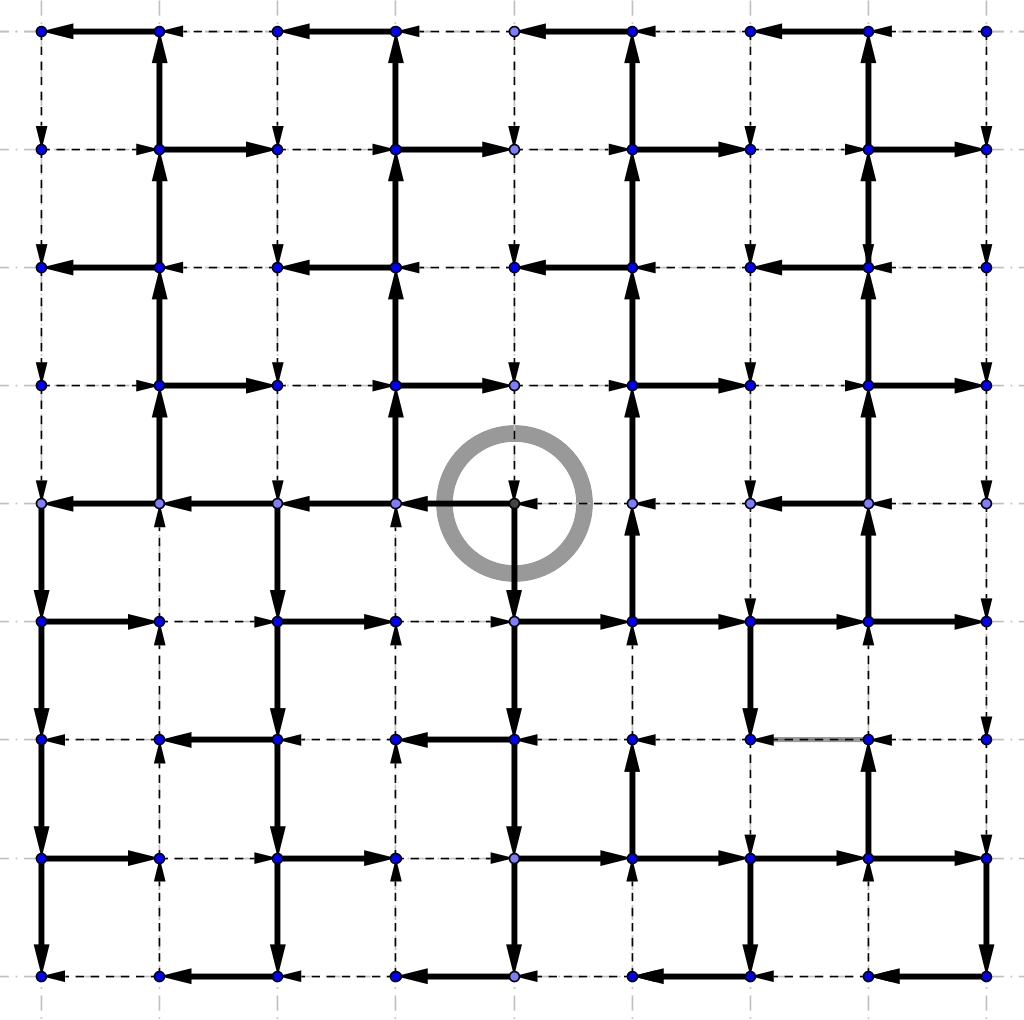
\includegraphics[scale=0.6]{manhattan/pics/even_even.png}
\end{frame}

\begin{frame}
    \frametitle{Разбор случаев}

    \begin{itemize}
        \item Для каждой точки посчитаем её штраф (на рисунке штраф, равный $0$, отмечен зелёным цветом, равный $2$ --- синим, равный $4$ --- красным.
    \end{itemize}
    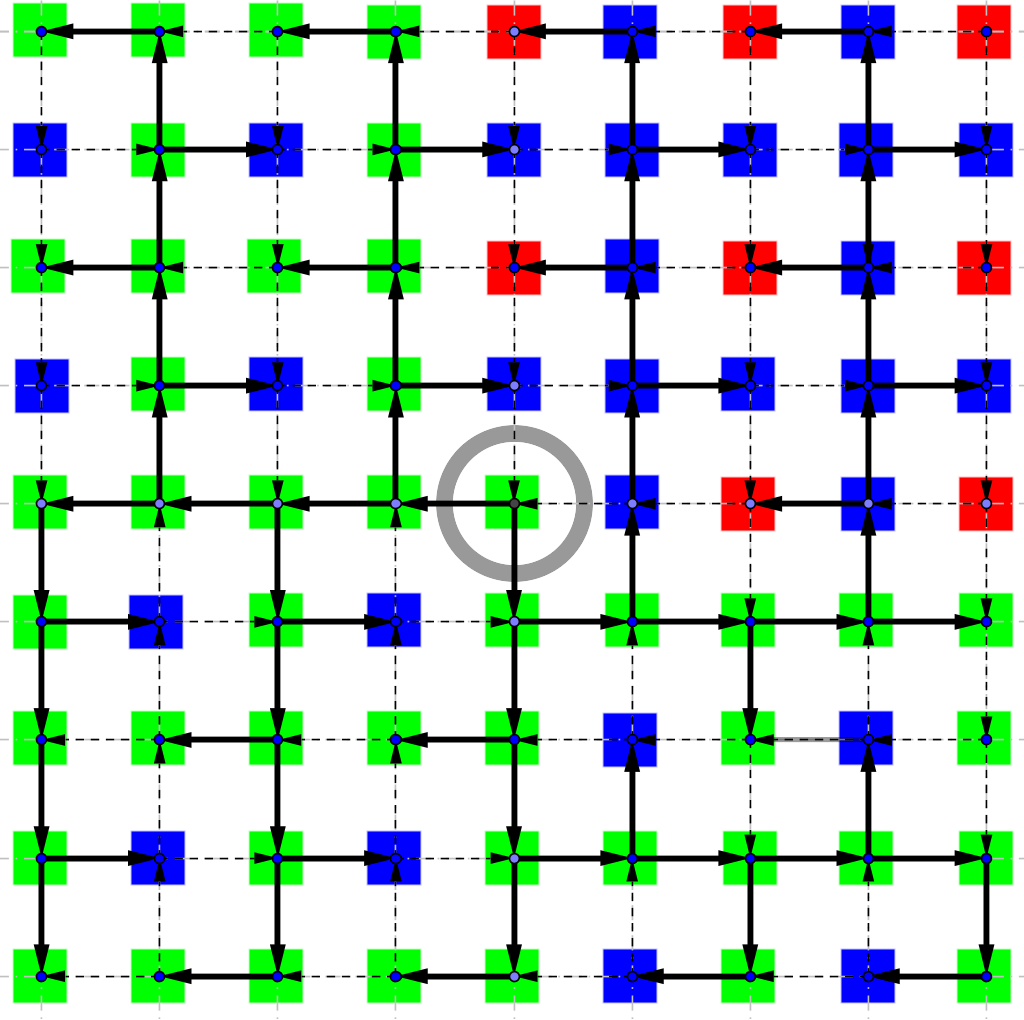
\includegraphics[scale=0.6]{manhattan/pics/even_even_penalty.png}
\end{frame}

\begin{frame}
    \frametitle{Разбор случаев}

    \begin{itemize}
        \item Заметим, что плоскость разбивается на четыре области, в каждой из которых штраф точки зависит только от чётности её координат.
    \end{itemize}
    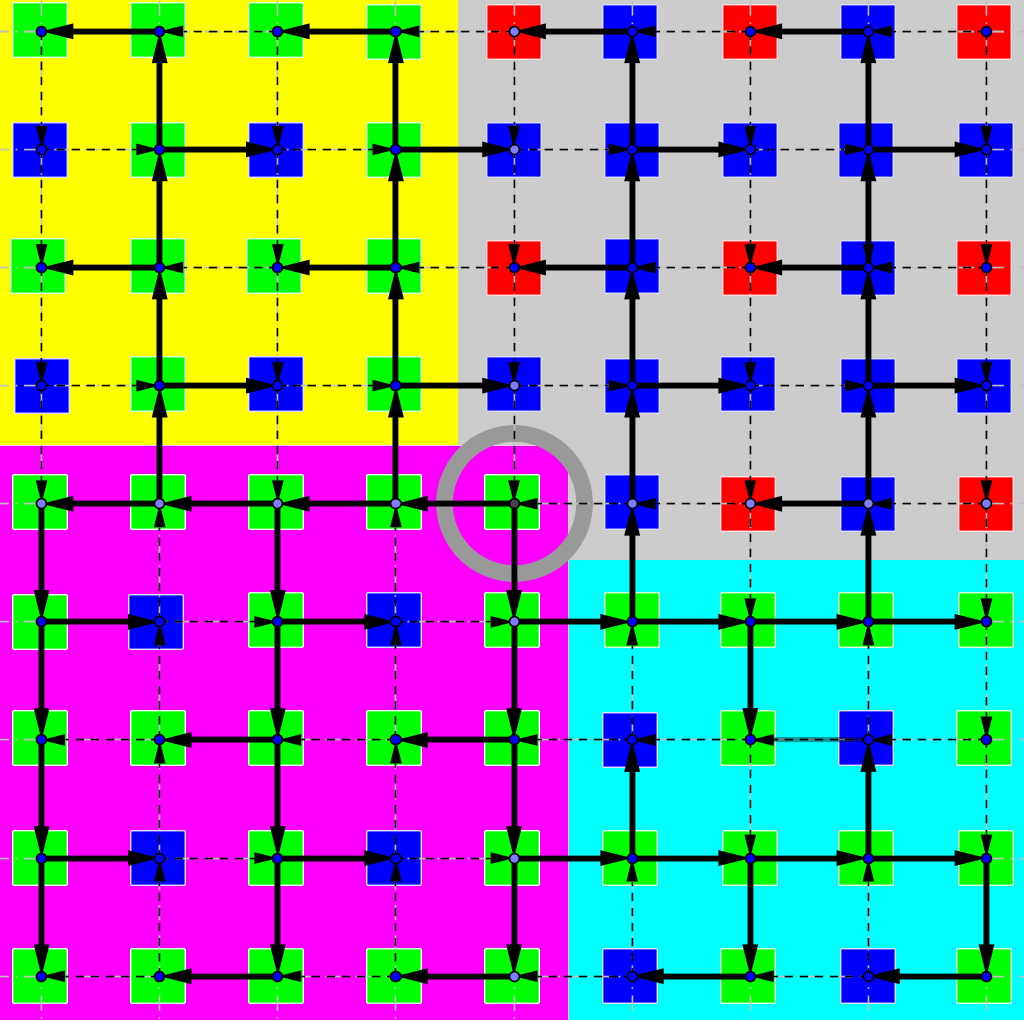
\includegraphics[scale=0.6]{manhattan/pics/even_even_regions.png}
\end{frame}

\begin{frame}
    \frametitle{Разбор случаев}

    \begin{itemize}
        \item Проверить, в какой области лежит точка~$F$ относительно точки~$S$.
        \item Посчитать её штраф в зависимости от полученной области и чётности координат.
        \item Прибавить к штрафу величину $|S_X-F_X| + |S_Y-F_Y|$.
        \item Это и есть ответ.
        \item Для остальных случаев, когда $S_X$ или $S_Y$ нечётные, рассуждения полностью аналогичны.
    \end{itemize}
\end{frame}

\begin{frame}
    \frametitle{Поиск в ширину}

    \begin{itemize}
        \item Можно было честно искать кратчайшее расстояние между точками с помощью, например, алгоритма поиска в ширину.
        \item Подробнее --- например, на сайте \url{http://informatics.msk.ru/} в разделе <<Алгоритмы на графах>>.
    \end{itemize}
\end{frame}

\begin{frame}
    \begin{center}
        \Huge Вопросы?
    \end{center}
\end{frame}

  \section{Задача <<Нью-Кэпитал>>}


\begin{frame}
    \begin{center}
        \Huge Задача <<Нью-Кэпитал>>
    \end{center}
    ~\\~\\
    \begin{center}
        Автор задачи: Олег~Мингалёв\\
        Автор условия: Елизавета~Игнатьева\\
        Автор тестов: Олег~Мингалёв
    \end{center}
\end{frame}

\subsection{Постановка задачи}

\begin{frame}
    \frametitle{Постановка задачи}

    \begin{itemize}
        \item На плоскости отмечены две точки $S$ и $F$: $(S_X, S_Y)$ и $(F_X, F_Y)$.
        \item Из точек с чётными $X$-координатами разрешено двигаться на $1$~влево.
        \item Из точек с нечётными $X$-координатами разрешено двигаться на $1$~вправо.
        \item Из точек с чётными $Y$-координатами разрешено двигаться на $1$~вниз.
        \item Из точек с нечётными $Y$-координатами разрешено двигаться на $1$~верх.
        \item Другие ходы запрещены
        \item За какое минимальное число ходов из точки $S$ можно попасть в точку $F$?
    \end{itemize}
\end{frame}

\subsection{Решение}

\begin{frame}
    \frametitle{Разбор случаев}

    \begin{itemize}
        \item Рассмотрим решение для случая, в котором $S_X$ и $S_Y$ чётные, остальные случаи разбираются аналогично.
    \end{itemize}
\end{frame}

\begin{frame}
    \frametitle{Разбор случаев}

    \begin{itemize}
        \item Если бы из точек можно было ходить в любую сторону, то ответом на задачу было бы число $D = |S_X-F_X| + |S_Y-F_Y|$.
        \item Понятно, что в решаемой нами задаче ответ не может быть меньше, чем $D$.
        \item Назовём штрафом точки $A: (X, Y)$ разность минимального количества ходов, необходимого для достижения точки~$A$ из точки~$S$ и величины $|S_X-Y| + |S_Y-Y|$.
    \end{itemize}
\end{frame}

\begin{frame}
    \frametitle{Разбор случаев}

    \begin{itemize}
        \item Нарисуем все кратчайшие пути из $S$.
    \end{itemize}
    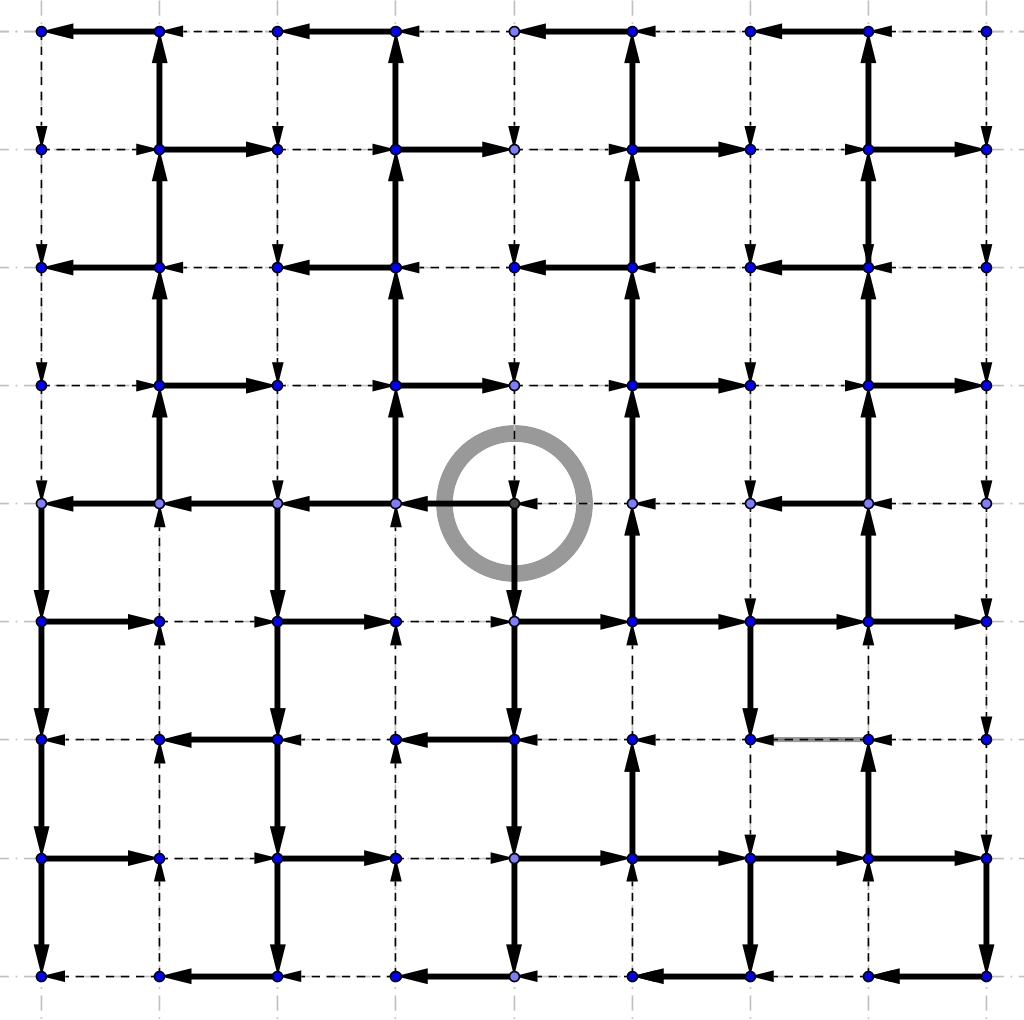
\includegraphics[scale=0.6]{manhattan/pics/even_even.png}
\end{frame}

\begin{frame}
    \frametitle{Разбор случаев}

    \begin{itemize}
        \item Для каждой точки посчитаем её штраф (на рисунке штраф, равный $0$, отмечен зелёным цветом, равный $2$ --- синим, равный $4$ --- красным.
    \end{itemize}
    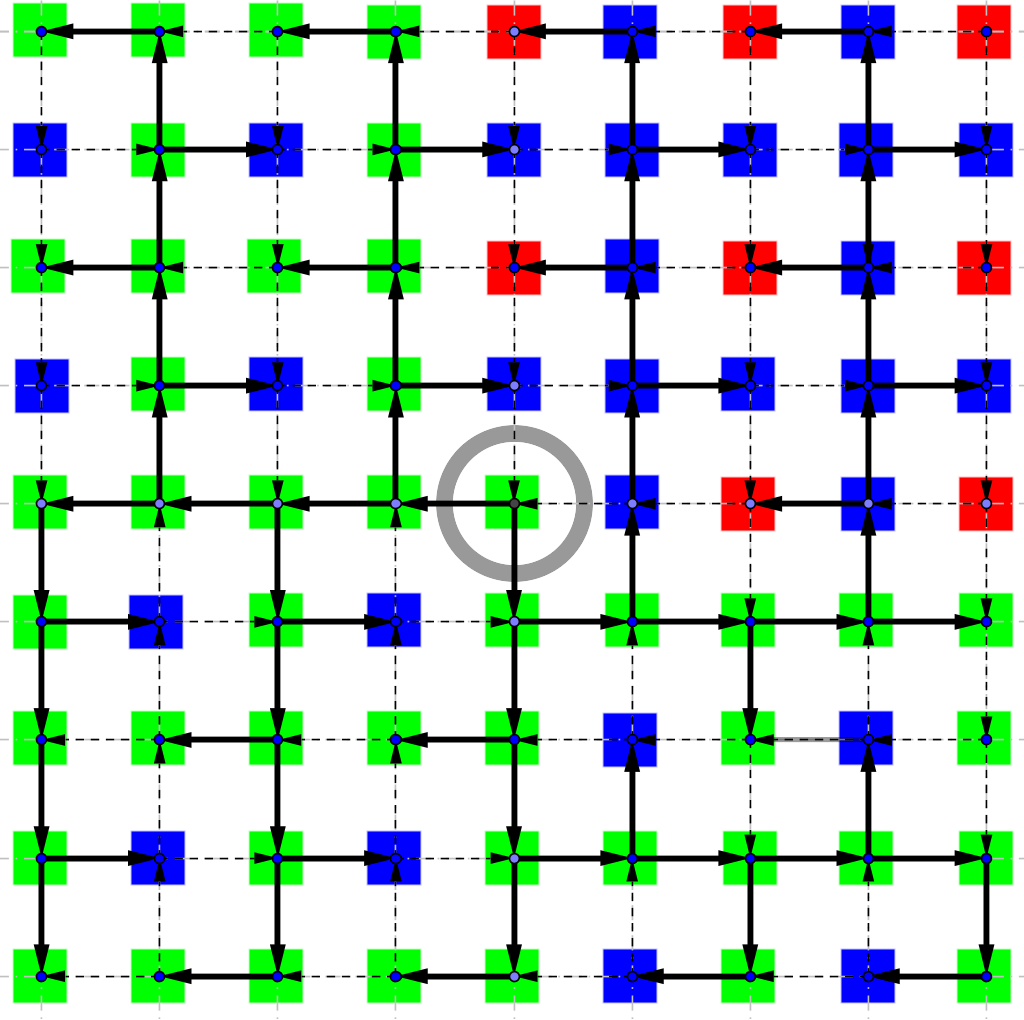
\includegraphics[scale=0.6]{manhattan/pics/even_even_penalty.png}
\end{frame}

\begin{frame}
    \frametitle{Разбор случаев}

    \begin{itemize}
        \item Заметим, что плоскость разбивается на четыре области, в каждой из которых штраф точки зависит только от чётности её координат.
    \end{itemize}
    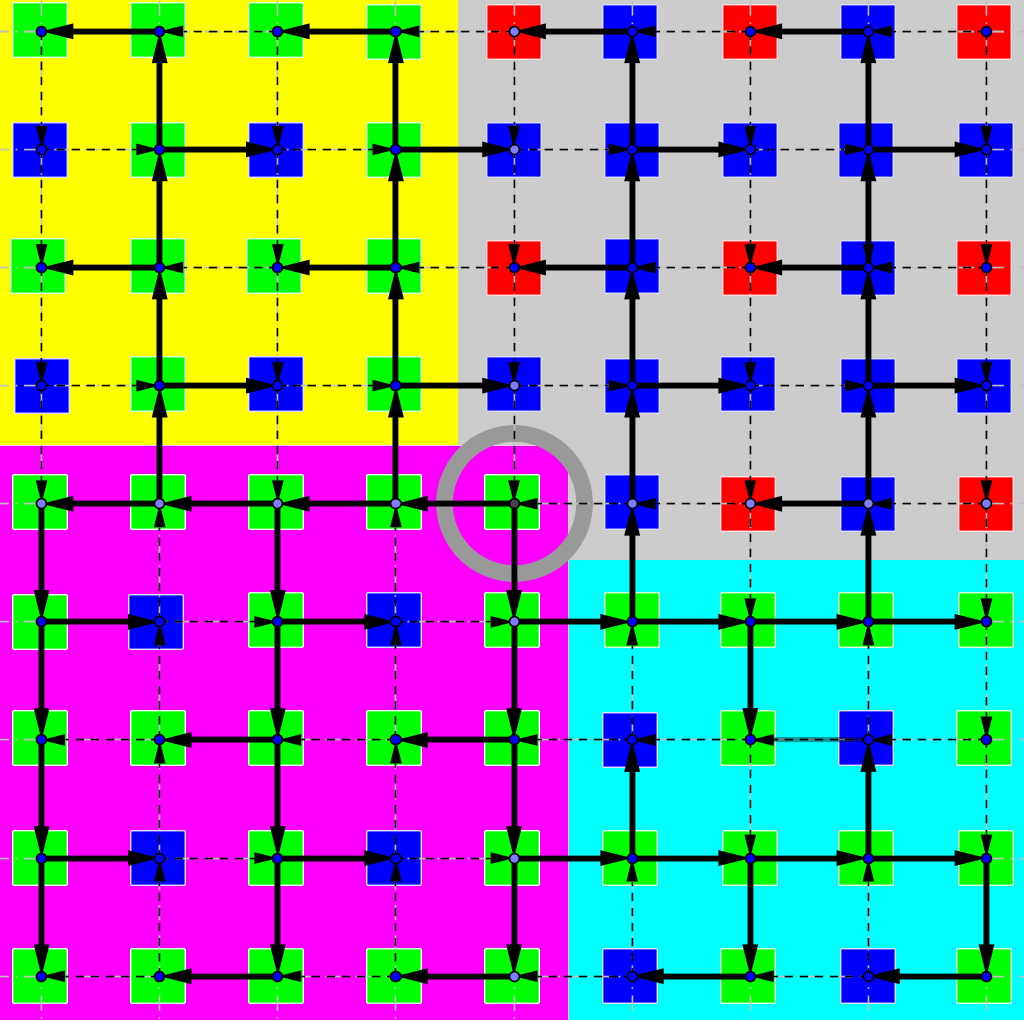
\includegraphics[scale=0.6]{manhattan/pics/even_even_regions.png}
\end{frame}

\begin{frame}
    \frametitle{Разбор случаев}

    \begin{itemize}
        \item Проверить, в какой области лежит точка~$F$ относительно точки~$S$.
        \item Посчитать её штраф в зависимости от полученной области и чётности координат.
        \item Прибавить к штрафу величину $|S_X-F_X| + |S_Y-F_Y|$.
        \item Это и есть ответ.
        \item Для остальных случаев, когда $S_X$ или $S_Y$ нечётные, рассуждения полностью аналогичны.
    \end{itemize}
\end{frame}

\begin{frame}
    \frametitle{Поиск в ширину}

    \begin{itemize}
        \item Можно было честно искать кратчайшее расстояние между точками с помощью, например, алгоритма поиска в ширину.
        \item Подробнее --- например, на сайте \url{http://informatics.msk.ru/} в разделе <<Алгоритмы на графах>>.
    \end{itemize}
\end{frame}

\begin{frame}
    \begin{center}
        \Huge Вопросы?
    \end{center}
\end{frame}

  \section{Задача <<Нью-Кэпитал>>}


\begin{frame}
    \begin{center}
        \Huge Задача <<Нью-Кэпитал>>
    \end{center}
    ~\\~\\
    \begin{center}
        Автор задачи: Олег~Мингалёв\\
        Автор условия: Елизавета~Игнатьева\\
        Автор тестов: Олег~Мингалёв
    \end{center}
\end{frame}

\subsection{Постановка задачи}

\begin{frame}
    \frametitle{Постановка задачи}

    \begin{itemize}
        \item На плоскости отмечены две точки $S$ и $F$: $(S_X, S_Y)$ и $(F_X, F_Y)$.
        \item Из точек с чётными $X$-координатами разрешено двигаться на $1$~влево.
        \item Из точек с нечётными $X$-координатами разрешено двигаться на $1$~вправо.
        \item Из точек с чётными $Y$-координатами разрешено двигаться на $1$~вниз.
        \item Из точек с нечётными $Y$-координатами разрешено двигаться на $1$~верх.
        \item Другие ходы запрещены
        \item За какое минимальное число ходов из точки $S$ можно попасть в точку $F$?
    \end{itemize}
\end{frame}

\subsection{Решение}

\begin{frame}
    \frametitle{Разбор случаев}

    \begin{itemize}
        \item Рассмотрим решение для случая, в котором $S_X$ и $S_Y$ чётные, остальные случаи разбираются аналогично.
    \end{itemize}
\end{frame}

\begin{frame}
    \frametitle{Разбор случаев}

    \begin{itemize}
        \item Если бы из точек можно было ходить в любую сторону, то ответом на задачу было бы число $D = |S_X-F_X| + |S_Y-F_Y|$.
        \item Понятно, что в решаемой нами задаче ответ не может быть меньше, чем $D$.
        \item Назовём штрафом точки $A: (X, Y)$ разность минимального количества ходов, необходимого для достижения точки~$A$ из точки~$S$ и величины $|S_X-Y| + |S_Y-Y|$.
    \end{itemize}
\end{frame}

\begin{frame}
    \frametitle{Разбор случаев}

    \begin{itemize}
        \item Нарисуем все кратчайшие пути из $S$.
    \end{itemize}
    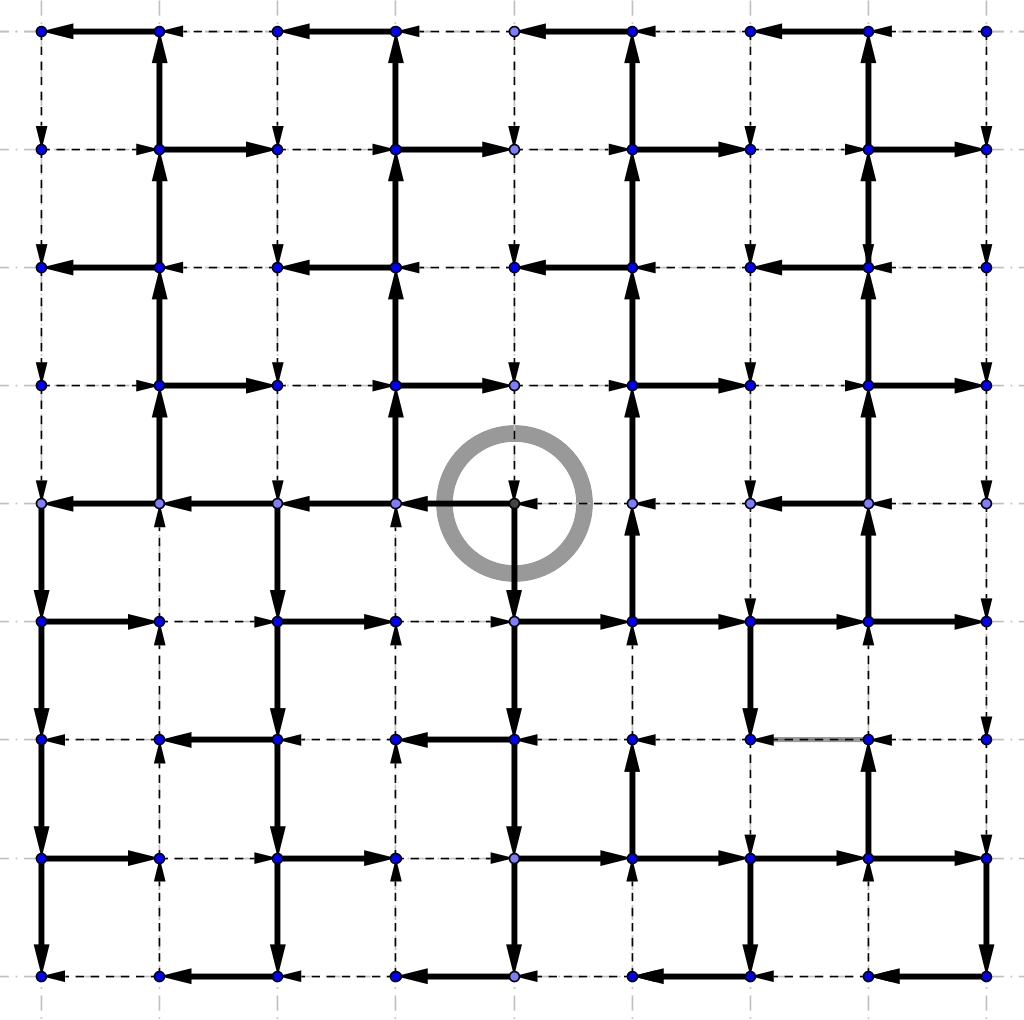
\includegraphics[scale=0.6]{manhattan/pics/even_even.png}
\end{frame}

\begin{frame}
    \frametitle{Разбор случаев}

    \begin{itemize}
        \item Для каждой точки посчитаем её штраф (на рисунке штраф, равный $0$, отмечен зелёным цветом, равный $2$ --- синим, равный $4$ --- красным.
    \end{itemize}
    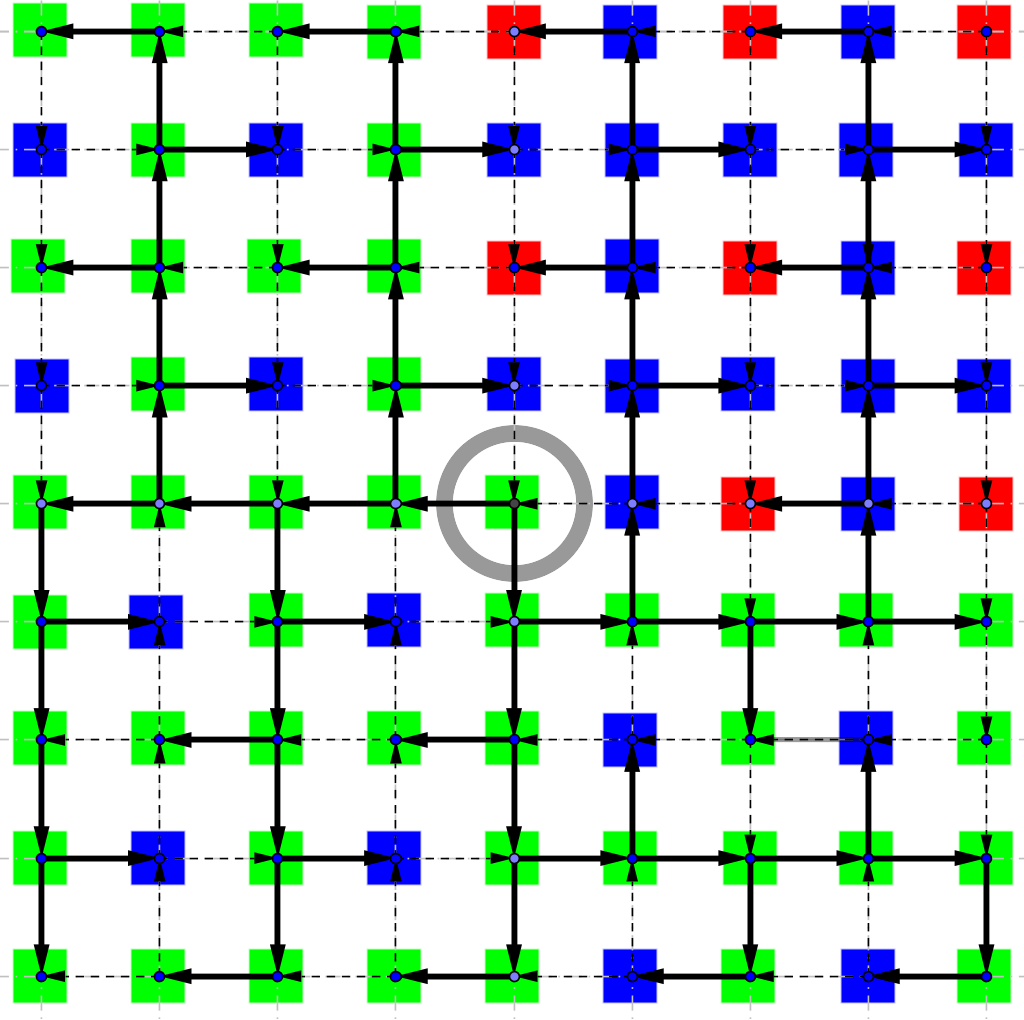
\includegraphics[scale=0.6]{manhattan/pics/even_even_penalty.png}
\end{frame}

\begin{frame}
    \frametitle{Разбор случаев}

    \begin{itemize}
        \item Заметим, что плоскость разбивается на четыре области, в каждой из которых штраф точки зависит только от чётности её координат.
    \end{itemize}
    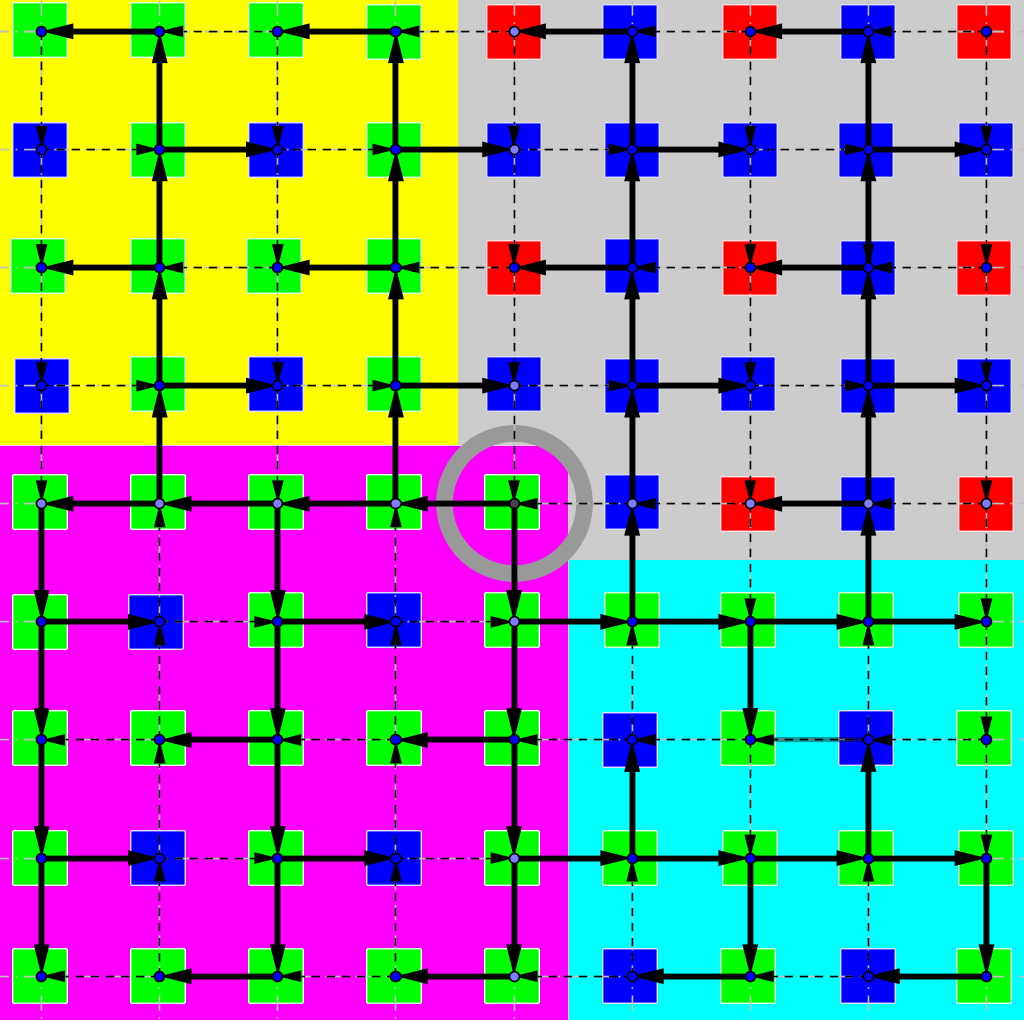
\includegraphics[scale=0.6]{manhattan/pics/even_even_regions.png}
\end{frame}

\begin{frame}
    \frametitle{Разбор случаев}

    \begin{itemize}
        \item Проверить, в какой области лежит точка~$F$ относительно точки~$S$.
        \item Посчитать её штраф в зависимости от полученной области и чётности координат.
        \item Прибавить к штрафу величину $|S_X-F_X| + |S_Y-F_Y|$.
        \item Это и есть ответ.
        \item Для остальных случаев, когда $S_X$ или $S_Y$ нечётные, рассуждения полностью аналогичны.
    \end{itemize}
\end{frame}

\begin{frame}
    \frametitle{Поиск в ширину}

    \begin{itemize}
        \item Можно было честно искать кратчайшее расстояние между точками с помощью, например, алгоритма поиска в ширину.
        \item Подробнее --- например, на сайте \url{http://informatics.msk.ru/} в разделе <<Алгоритмы на графах>>.
    \end{itemize}
\end{frame}

\begin{frame}
    \begin{center}
        \Huge Вопросы?
    \end{center}
\end{frame}

  \section{Задача <<Нью-Кэпитал>>}


\begin{frame}
    \begin{center}
        \Huge Задача <<Нью-Кэпитал>>
    \end{center}
    ~\\~\\
    \begin{center}
        Автор задачи: Олег~Мингалёв\\
        Автор условия: Елизавета~Игнатьева\\
        Автор тестов: Олег~Мингалёв
    \end{center}
\end{frame}

\subsection{Постановка задачи}

\begin{frame}
    \frametitle{Постановка задачи}

    \begin{itemize}
        \item На плоскости отмечены две точки $S$ и $F$: $(S_X, S_Y)$ и $(F_X, F_Y)$.
        \item Из точек с чётными $X$-координатами разрешено двигаться на $1$~влево.
        \item Из точек с нечётными $X$-координатами разрешено двигаться на $1$~вправо.
        \item Из точек с чётными $Y$-координатами разрешено двигаться на $1$~вниз.
        \item Из точек с нечётными $Y$-координатами разрешено двигаться на $1$~верх.
        \item Другие ходы запрещены
        \item За какое минимальное число ходов из точки $S$ можно попасть в точку $F$?
    \end{itemize}
\end{frame}

\subsection{Решение}

\begin{frame}
    \frametitle{Разбор случаев}

    \begin{itemize}
        \item Рассмотрим решение для случая, в котором $S_X$ и $S_Y$ чётные, остальные случаи разбираются аналогично.
    \end{itemize}
\end{frame}

\begin{frame}
    \frametitle{Разбор случаев}

    \begin{itemize}
        \item Если бы из точек можно было ходить в любую сторону, то ответом на задачу было бы число $D = |S_X-F_X| + |S_Y-F_Y|$.
        \item Понятно, что в решаемой нами задаче ответ не может быть меньше, чем $D$.
        \item Назовём штрафом точки $A: (X, Y)$ разность минимального количества ходов, необходимого для достижения точки~$A$ из точки~$S$ и величины $|S_X-Y| + |S_Y-Y|$.
    \end{itemize}
\end{frame}

\begin{frame}
    \frametitle{Разбор случаев}

    \begin{itemize}
        \item Нарисуем все кратчайшие пути из $S$.
    \end{itemize}
    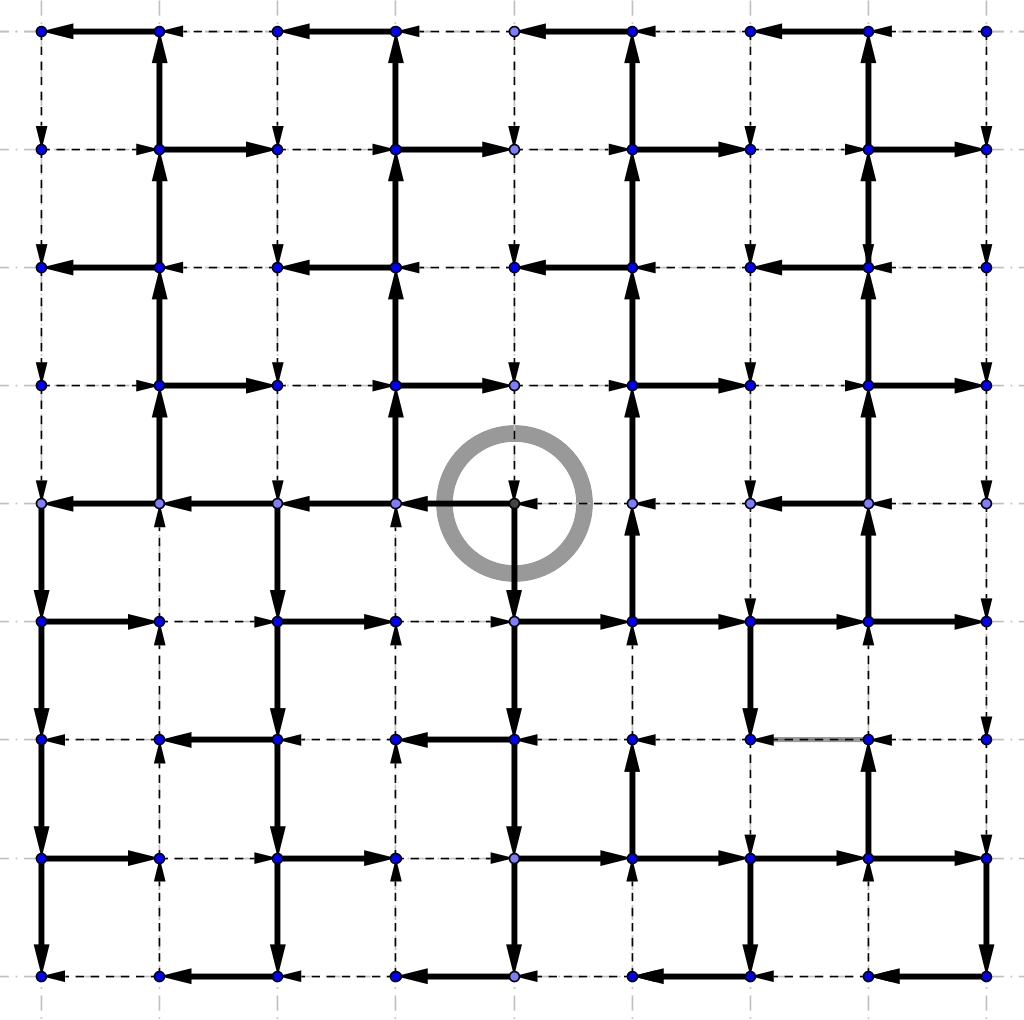
\includegraphics[scale=0.6]{manhattan/pics/even_even.png}
\end{frame}

\begin{frame}
    \frametitle{Разбор случаев}

    \begin{itemize}
        \item Для каждой точки посчитаем её штраф (на рисунке штраф, равный $0$, отмечен зелёным цветом, равный $2$ --- синим, равный $4$ --- красным.
    \end{itemize}
    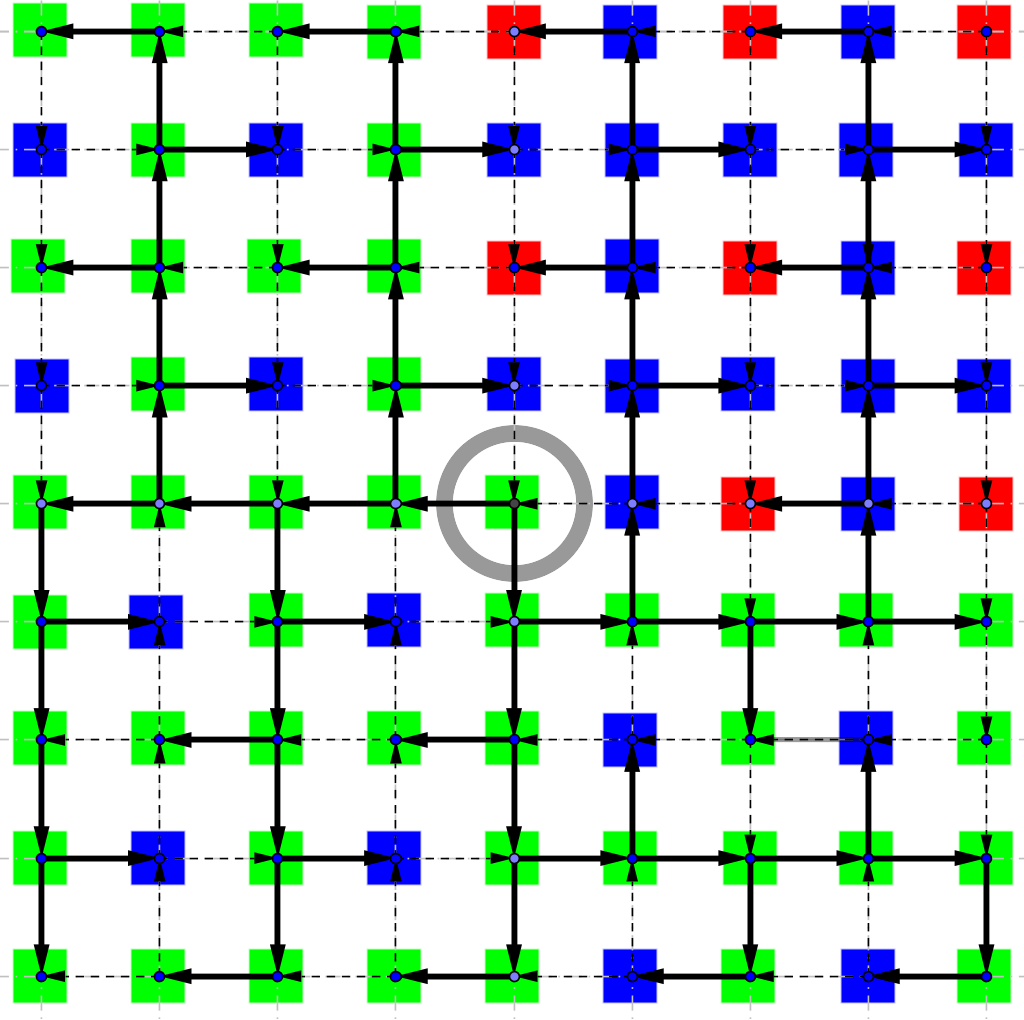
\includegraphics[scale=0.6]{manhattan/pics/even_even_penalty.png}
\end{frame}

\begin{frame}
    \frametitle{Разбор случаев}

    \begin{itemize}
        \item Заметим, что плоскость разбивается на четыре области, в каждой из которых штраф точки зависит только от чётности её координат.
    \end{itemize}
    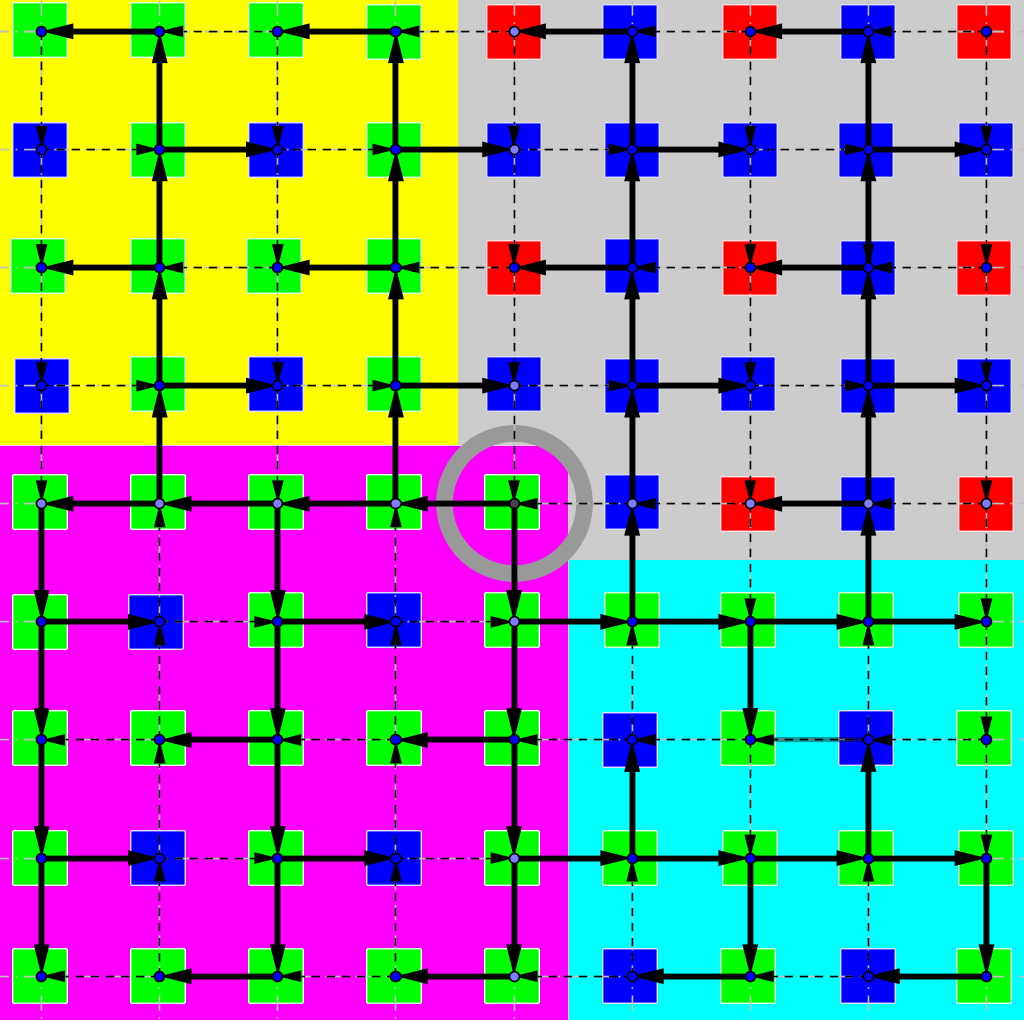
\includegraphics[scale=0.6]{manhattan/pics/even_even_regions.png}
\end{frame}

\begin{frame}
    \frametitle{Разбор случаев}

    \begin{itemize}
        \item Проверить, в какой области лежит точка~$F$ относительно точки~$S$.
        \item Посчитать её штраф в зависимости от полученной области и чётности координат.
        \item Прибавить к штрафу величину $|S_X-F_X| + |S_Y-F_Y|$.
        \item Это и есть ответ.
        \item Для остальных случаев, когда $S_X$ или $S_Y$ нечётные, рассуждения полностью аналогичны.
    \end{itemize}
\end{frame}

\begin{frame}
    \frametitle{Поиск в ширину}

    \begin{itemize}
        \item Можно было честно искать кратчайшее расстояние между точками с помощью, например, алгоритма поиска в ширину.
        \item Подробнее --- например, на сайте \url{http://informatics.msk.ru/} в разделе <<Алгоритмы на графах>>.
    \end{itemize}
\end{frame}

\begin{frame}
    \begin{center}
        \Huge Вопросы?
    \end{center}
\end{frame}

% etc
\end{document}
